% ---------------------------------------------------------------------
% --- Arquivo principal e os demais serao os dos capitulos.
% --- EXPRESSÔES ENTRE <> DEVERÂO SER COMPLETADAS COM A INFORMAÇÂO ESPECÌFICA DO TRABALHO 
% ---------------------------------------------------------------------

% Atualizado para atender as normas ABNT por Mônica da Silva (04/11/2021)

%configuração da entrada 
    % 12pt, 	% tamanho da fonte
    %openright, % capítulos começam em pág ímpar (insere página vazia caso preciso)
    % oneside, %% IMPRESSÃO dos elementos textuais e pós-textuais: oneside (apenas no anverso) ou twoside (anverso e verso, se mais de 100 p.) (insere páginas em branco).
    % a4paper, % tamanho do papel. 
    % english, % idioma adicional para hifenização
   	%english,			% idioma adicional para hifenização
	%french,				% idioma adicional para hifenização
	%spanish,			% idioma adicional para hifenização
	%brazil,				% o último idioma é o principal do documento

\documentclass[ruledheader, 12pt, openright, a4paper, oneside, english, brazil]{PPGC_UFF}



%---pacotes para hiphenizacao e acentuacao em portugues
\usepackage[brazil]{babel}
\usepackage[T1]{fontenc}
\usepackage[utf8]{inputenc}	
%\usepackage[latin1]{inputenc}
\usepackage{csquotes}


%--- pacote para figuras
\usepackage{epsf, subfigure}
\usepackage[dvips]{epsfig,graphicx}
\usepackage{chngcntr} %configuração dos padrões numéricos das Figuras e Tabelas
\counterwithout{figure}{chapter} %formata figura para padrão: Figura 1.
\counterwithout{table}{chapter} %formata tabela para padrão: Tabela 1.


%--- pacote de simbolos
\usepackage{pifont,textcomp,latexsym}

%--- simbolos matematicos
\usepackage{amssymb,amstext,amsthm,icomma,amsmath}

%--- pacote para gerar pseudo-codigo
\usepackage{algorithm}
\usepackage{algorithmic}
\floatname{algorithm}{Algoritmo}

%--- outros pacotes
\usepackage{url}
\usepackage{longtable}
\usepackage{lscape}
\usepackage{quoting}
\usepackage{csvsimple} %criação da tabela do apêndice A

%Tabela Colorida
\usepackage{bigdelim,booktabs, colortbl, longtable, multirow, multicol,rotating }



%%===============================================================================
%% INICIO do Pacotes - Lista de abreviaturas, siglas e acrônimos
%%===============================================================================
		
% Modo "file": utiliza os termos definidos no arquivo acronimos.tex
%  1) Inserção tabular da listas
%  2) Controle da ordem de apresentação das listas
%  3) Não é preciso referenciar no texto
% nonumberlist, %do not show page numbers
% acronym,      %generate acronym listing   -> Not used in this example (see line with)
% toc,          % Inclui a abreviatura no sumário e conta pagina
% section]      %use section level for toc entries
\usepackage[acronym,nopostdot,shortcuts, nonumberlist]{glossaries}


\makeglossaries
\newacronym{ONU}{ONU}{Organização das Nações Unidas}
\newacronym{ACR}{ACR}{Acronimos}
\newacronym{cor}{COR}{Centro de Operações do Rio}
\newacronym{cnn}{\textit{CNN}}{\textit{Convolutional Neural Network}}
% Trabalhos Relacionados
\newacronym{knn}{\textit{k-NN}}{\textit{k-Nearest Neighbours}}
\newacronym{svm}{\textit{SVM}}{\textit{Support Vector Machine}}
\newacronym{bovw}{\textit{BoVW}}{\textit{Bag of Visual Words}}
\newacronym{ml}{\textit{ML}}{\textit{Machine Learning}}
%
\newacronym{vit}{\textit{ViT}}{\textit{Visual Transformer}}
\newacronym{sgd}{\textit{SGD}}{\textit{Stochastic Gradient Descent}}
\newacronym{vgg}{\textit{VGG}}{\textit{Visual Geometry Group}}
\newacronym{mlp}{\textit{MLP}}{\textit{Multilayer Perceptron}}
%
\newacronym{adam}{\textit{ADAM}}{\textit{Adaptive Moment Estimation}}
\newacronym{nadam}{\textit{NADAM}}{\textit{Nesterov-accelerated Adaptive Moment Estimation}}
\newacronym{efd}{\textit{EFD}}{European Flood Dataset}


%%===============================================================================
%% FIM do Pacotes Lista de abreviaturas, siglas e acrônimos
%%===============================================================================

%%===============================================================================
%% Configuração das citações e personalização 
%%===============================================================================

% Os pacotes abaixo só podem ser usados juntamente com o pacote ABNT abaixo e na ordem atual. 
% Esse conjunto de pacotes permite que as citações fiquem na cor azul e sejam usadas como link para as referencias. 
\usepackage[bookmarksopen=true,
            linktoc=page, 
            colorlinks=true,  %ativa a cor do link na referencia
            linkcolor=blue, %muda a cor do link na referencia \ref{} números de tabelas, figuras, seções, sumário etc. 
            citecolor=blue, % muda a cor das citações \cite \textcite
            filecolor=magenta, 
            urlcolor=blue, %muda a cor da url \url no texto e ref. bibliográfica
            ]{hyperref}


\usepackage[ %mais informações de personalização das referencias olhar nos arquivos PDF na pasta MANUAIS OU https://www.overleaf.com/learn/latex/Biblatex_bibliography_styles
    %style = abnt, % Sistema alfabético
    style = abnt-numeric, % Sistema numérico
    %style = abnt-ibid, % Notas de referência
    language=brazil,
    backend=biber,
    citestyle = numeric,
    %minbibnames=1,
    %maxbibnames=1,
]{biblatex}

\addbibresource{bibliografia.bib} % A biblioteca para ser utilizada na dissertação/tese.
\DefineBibliographyStrings{brazil}{%
  pages = {pp\adddot},
}
%%===============================================================================
%% FIM da configuração das citações e personalização 
%%===============================================================================

\hyphenation{
a-de-qua-da-men-te 
di-men-sio-na-men-to 
}

%---------usando tipo de fonte padrão  
% mathptmx (títulos sem negrito) ou ptm (títulos negrito)  - Times - Padrão 
% ugq (títulos negrito) - Arial 
%% --  Padrão do template é: ptm  -- %%
\renewcommand{\ABNTchapterfont}{\bfseries\fontfamily{ptm}\fontseries{b}\selectfont} 
\renewcommand{\ABNTsectionfont}{\bfseries\fontfamily{ptm}}


% --- -----------------------------------------------------------------
% --- Documento Principal.
% --- -----------------------------------------------------------------

\begin{document}


% --- -----------------------------------------------------------------
% --- Titulo, abstract, dedicatórias e agradecimentos.
% --- Índice geral, lista de figuras e tabelas.
% --- -----------------------------------------------------------------
% Atualizado para atender as normas ABNT por Mônica da Silva (04/11/2021)

% --- -----------------------------------------------------------------
% --- Elementos usados na Capa e na Folha de Rosto.
% --- EXPRESSÔES ENTRE <> DEVERÂO SER COMPLETADAS COM A INFORMAÇÂO ESPECÍFICA DO TRABALHO
% --- E OS SÌMBOLOS <> DEVEM SER RETIRADOS 
% --- -----------------------------------------------------------------
\autor{André Fernandes Gonçalves} % deve ser escrito em maiúsculo

\titulo{Classificação de Alagamentos na Cidade do Rio de Janeiro através de Visão Computacional}

\instituicao{UNIVERSIDADE FEDERAL FLUMINENSE}

\orientador{Aura Conci}

%\coorientador{<NOME DO COORIENTADOR>} % se nao existir co-orientador apague essa linha

\local{NITER\'{O}I}

\data{2025} % ano da defesa

\comentario{Dissertação de Mestrado apresentada ao Programa de P\'{o}s-Gradua\c{c}\~{a}o em Computa\c{c}\~{a}o da \mbox{Universidade} Federal Fluminense como requisito parcial para a obten\c{c}\~{a}o do Grau de \mbox{Mestre em Computa\c{c}\~{a}o}. \'{A}rea de concentra\c{c}\~{a}o: \mbox{Computa\c{c}\~{a}o}} %preencha com a sua área de concentração


% --- -----------------------------------------------------------------
% --- Capa. (Capa externa, aquela com as letrinhas douradas)(Obrigatório)
% --- ----------------------------------------------------------------
\capa

% --- -----------------------------------------------------------------
% --- Folha de rosto. (Obrigatório)
% --- ----------------------------------------------------------------
\folhaderosto

% --- -----------------------------------------------------------------
% --- Ficha catalográfica obrigatória na versão final. (Obrigatório)
% --- ----------------------------------------------------------------

\begin{figure}[!ht]
   \centering
   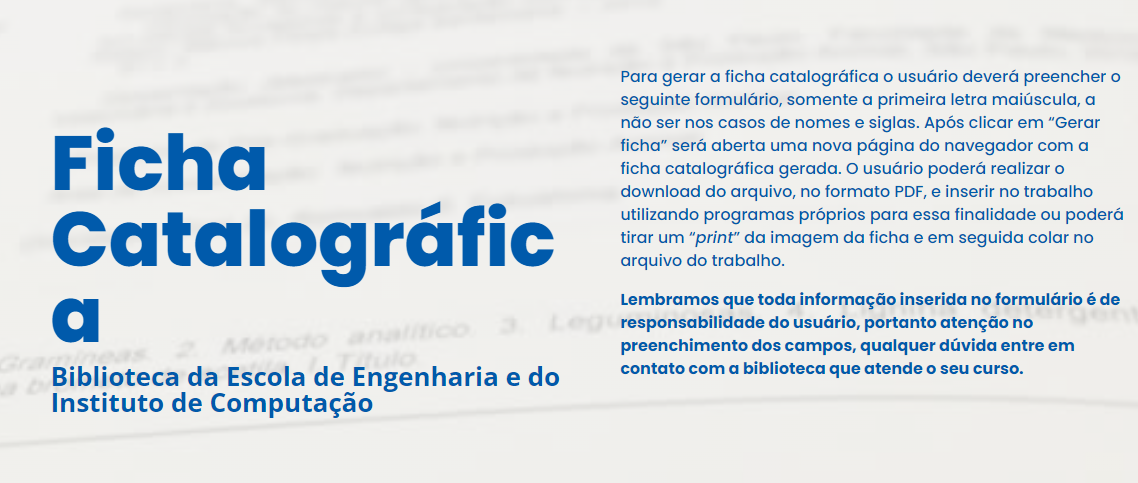
\includegraphics[width=1\linewidth]{capitulos/figuras/ficha_catalografica.png}
   \caption{Local da ficha catalográfica}
\end{figure}

\cleardoublepage


\pagestyle{ruledheader}
\setcounter{page}{1}
\pagenumbering{roman}

% --- -----------------------------------------------------------------
% --- Termo de aprovação. (Obrigatório)
% --- ----------------------------------------------------------------
\cleardoublepage
\thispagestyle{empty}

\vspace{-60mm}

\begin{center}
   {\large ANDRÉ FERNANDES GONÇALVES}\\
   \vspace{7mm}

   \uppercase{Classificação de Alagamentos na Cidade do Rio de Janeiro através de Visão Computacional}\\
  \vspace{10mm}
\end{center}

\noindent
\begin{flushright}
\begin{minipage}[t]{8cm}

Dissertação de Mestrado apresentada ao Programa de P\'{o}s-Gradua\c{c}\~{a}o em Computa\c{c}\~{a}o da Universidade Federal Fluminense como requisito parcial para a obten\c{c}\~{a}o do \mbox{Grau} de Mestre em Computa\c{c}\~{a}o. \'{A}rea de concentra\c{c}\~{a}o: \mbox{Computa\c{c}\~{a}o} %preencha com a sua área de concentração

\end{minipage}
\end{flushright}
\vspace{1.0 cm}
\noindent
Aprovada em <MES> de 2025. \\
\begin{flushright}
 % \parbox{11cm}
  {
  \begin{center}
  BANCA EXAMINADORA \\
  \vspace{6mm}
  \rule{11cm}{.1mm} \\
    Prof. Aura Conci - Orientadora, UFF \\
    \vspace{6mm}
  \rule{11cm}{.1mm} \\
    Prof. Leandro Augusto Frata Fernandes, UFF\\
    \vspace{6mm}
  \rule{11cm}{.1mm} \\
    Prof. Flávia Cristina Bernardini, UFF\\
  \vspace{4mm}
  \rule{11cm}{.1mm} \\
    Prof. Aristófanes Corrêa Silva\\
    \vspace{6mm}
  \rule{11cm}{.1mm} \\
    Prof. Raul Queiroz Feitosa, PUC\\
  \vspace{6mm}
  \end{center}
  }
\end{flushright}
\begin{center}
  \vspace{4mm}
  Niter\'{o}i \\
  %\vspace{6mm}
  2025

\end{center}

% --- -----------------------------------------------------------------
% --- Dedicatoria.(Opcional)
% --- -----------------------------------------------------------------
\cleardoublepage
\thispagestyle{empty}
\vspace*{200mm}

\begin{flushright}
{\em 
    Aos meus pais, que me apoiaram ao longo da minha jornada.
}
\end{flushright}
\newpage


% --- -----------------------------------------------------------------
% --- Agradecimentos.(Opcional)
% --- -----------------------------------------------------------------
\pretextualchapter{Agradecimentos}
\hspace{5mm}
A minha orientadora, Aura Conci, que me ajudou em todo o caminho e sempre confiou em mim.

A UFF e a CAPES, pela bolsa que me ajudou durante meus estudos do mestrado.

A Luis Rezende e Otávio Flaeschen pela ajuda na criação do conjunto de dados.



% --- -----------------------------------------------------------------
% --- Resumo em português.(Obrigatório)
% --- -----------------------------------------------------------------
\begin{resumo}

%Elemento obrigatório, constituído de uma sequência de frases concisas e objetivas e não de uma simples enumeração de tópicos, não ultrapassando 500 palavras ABNT NBR 6028:2003.

Este trabalho teve como objetivo desenvolver uma abordagem inicial para a classificação automática de alagamentos da cidade do Rio de Janeiro.
Para isso, este trabalho primeiramente criou um conjunto de dados original composto de 4620 separadas em 78\% para treino e 22\% para validação.
Este conjunto de dados foi montado com imagens da própria cidade do Rio ao longo de diferentes meses, em diferentes horas do dia e em diferentes níveis de alagamento.
Após o conjunto de dados ser devidamente analisado e montado de forma equilibrada, cinco arquiteturas de redes neurais foram avaliadas nesse conjunto de dados. 
Essas arquiteturas foram escolhidas de acordo com trabalhos da literatura com temática relacionada ao problema abordado.
Após o treinamento das arquiteturas \acrshort{vgg}-19, \textit{Inception}, \textit{DenseNet}, \textit{MobileNetV2}, e \textit{Visual Transformer} para o problema de classificação de imagem, 
o \textit{Visual Transformer} obteve melhor resultado e também foi analisado com diferentes níveis de iluminação, três diferentes otimizadores além de investigar se o aumento 
na quantidade de imagens de treino traria ganhos compensadores e validar o seu desempenho em outros dois conjuntos de dados.
Ao final, o \textit{Visual Transformer} foi melhor modelo com com acurácia de 82,6\% no conjunto de dados original.

\textbf{descrever o github junto com o conjunto de dados.}

{\hspace{-8mm} \bf{Palavras-chave}}: Visão Computacional, Rede Neural Convolucional, \textit{Visual Transformer}, Classificação, Alagamento.

\end{resumo}

% --- -----------------------------------------------------------------
% --- Resumo em língua estrangeira.(Obrigatório)
% --- -----------------------------------------------------------------
\begin{abstract}

%Elemento obrigatório, em língua estrangeira, com as mesmas características do resumo em língua vernácula (ABNT, 2005).
%O resumo deve ser redigido na terceira pessoa do singular, com verbo na voz ativa, não ultrapassando uma página ou 500 palavras, segundo a ABNT NBR 6028). Evitando-se ouso de parágrafos no meio do resumo, assim como fórmulas, equações e símbolos. Iniciar o resumo situando o trabalho no contexto geral, apresentar os objetivos, descrever a metodologia utilizada, relatar a contribuição própria, comentar os resultados obtidos e finalmente apresentaras conclusões mais importantes do trabalho.

This study aimed to develop an initial approach for the automatic classification of flooding events in the city of Rio de Janeiro.  
To achieve this, an original dataset was first created, consisting of 4,620 images, which were split into 78% for training and 22% for validation. This dataset was composed of images captured in different months, at various times of the day, and under different flooding levels within the city of Rio de Janeiro.  
After ensuring that the dataset was properly analyzed and balanced, five neural network architectures were evaluated on this dataset. These architectures were selected based on related works in the literature that address similar classification problems.  
Following the training of the \acrshort{vgg}-19, \textit{Inception}, \textit{DenseNet}, \textit{MobileNetV2}, and \textit{Visual Transformer} architectures for the image classification task, the \textit{Visual Transformer} achieved the best performance. Consequently, further analysis was conducted on this model, including evaluations under different lighting conditions, with three different optimizers, as well as an investigation into whether increasing the number of training images would yield significant improvements. Additionally, its performance was validated on two other datasets.  
Ultimately, the \textit{Visual Transformer} emerged as the best-performing model, achieving an accuracy of 82.6% on the original dataset.

{\hspace{-8mm} \bf{Keywords}}: Computer Vision, Convolutional Neural Network, \textit{Visual Transformer}, Classification, Flooding

\end{abstract}

% --- -----------------------------------------------------------------
% --- Lista de figuras.(Opcional)
% --- -----------------------------------------------------------------
%\cleardoublepage
\listoffigures



% --- -----------------------------------------------------------------
% --- Lista de tabelas.(Opcional)
% --- -----------------------------------------------------------------
\cleardoublepage
%\label{pag:last_page_introduction}
\listoftables
\cleardoublepage

% --- -----------------------------------------------------------------
% --- Lista de abreviatura.(Opcional)
%Elemento opcional, que consiste na relação alfabética das abreviaturas e siglas utilizadas no texto, seguidas das %palavras ou expressões correspondentes grafadas por extenso. Recomenda-se a elaboração de lista própria para cada %tipo (ABNT, 2005).
% --- ----------------------------------------------------------------

\cleardoublepage
\printglossary[type=\acronymtype,title={Lista de Abreviaturas e Siglas}]
\cleardoublepage


% --- -----------------------------------------------------------------
% --- Sumario.(Obrigatório)
% --- -----------------------------------------------------------------

\pagestyle{ruledheader}
\tableofcontents
\pagebreak %na pasta capítulos

% --- -----------------------------------------------------------------
% --- Inserção dos capítulos.
% --- todos os arquivos estão na pasta capítulos
% --- -----------------------------------------------------------------

\setcounter{page}{1} %parâmetros da contagem de paginas.
\pagenumbering{arabic} %padrão de números de paginas em arábico (1,2,3) 
\setcounter{page}{12} %inicia a contagem das paginas 12 - folha de rosto e considera a pagina da 

\pagestyle{ruledheader}

%%%% CAPÍTULO 1 - INTRODUÇÃO
%%
%% Deve apresentar uma visão global da pesquisa, 
%% incluindo: breve histórico, importância e
%% justificativa da escolha do tema, delimitações
%% do assunto, formulação de hipóteses e objetivos
%% da pesquisa e estrutura do trabalho.

% Perguntas que podem guiar a introdução - não necessariamente irá ter a resposta para tudo, isso depende da área.
% 1 - Qual é o contexto em que seu trabalho está inserido?
% 2 - Qual é o problema que motiva a existência deste trabalho?
% 3 - Qual é a visão geral da literatura sobre o problema e como é tratado
% 4 - Por que a solução na literatura não é o suficiente para ?
% 5 - Como seu trabalho trata o problema ?
% 6 - como seu trabalho foi avaliado para comprovar que tratou adequadamente o problema?
% 7 - De forma geral quais foram os resultados ?
% 8 - Quais foram as contribuições do seu trabalho?
% 9 -  Como o restante da Dissertação ou Tese está organizada ?


\chapter{Introdução}\label{cap:introducao}

A alta urbanização global, em conjunto com as rápidas mudanças climáticas globais, tem intensificado a ocorrência e o impacto de desastres ambientais.
Dentre estes, alagamentos representam 40\% dos desastres e, desde o ano 2000, desastres relacionados a alagamentos têm aumentado em 134\% em comparação às décadas anteriores \cite{gar2025}.

O Brasil, em específico, pode ter impacto anual de até 50 milhões de dólares em perdas econômicas sobre infraestrutura crítica vinda de alagamentos e ciclones \cite{gar2025map}.
Em 2024, o país registrou 140 ocorrências de desastres relacionados a alagamentos, desabrigando ou desalojando 30.000 brasileiros e trazendo prejuízos públicos e privados de 47 milhões de reais \cite{addb2025}.
De acordo com análise da Defesa Civil do Rio de Janeiro, em 2019, mais de milhões de pessoas foram diretamente afetadas por inundações, alagamentos e enxurradas nas regiões da capital, metropolitana e baixada fluminense \cite{defesacivil2019}.
Em reportagem de O Globo, estima-se que as chuvas intensas no período de 2019 a 2023 causaram prejuízos de 2,9 bilhões de reais ao estado do Rio de Janeiro.

Segundo a Classificação e Codificação Brasileira de Desastres, alagamento é uma extrapolação da capacidade de escoamento de sistemas de drenagem urbana e consequente acúmulo de água em ruas,
calçadas ou outras infraestruturas urbanas, em decorrência de precipitações intensas. Esse acúmulo afeta diretamente o trânsito de veículos e pedestres, principalmente em áreas urbanas,
tornando imprescindível a vigilância de áreas possivelmente afetadas por alagamentos.

Parte da insuficiência do sistema de drenagem urbana do Rio de Janeiro vem do fato de que foi construído em grande parte no início do século XX,
não sendo projetado para suportar os volumes de precipitação atualmente registrados, intensificados pelas mudanças climáticas e pela expansão urbana não planejada \cite{planodiretor}.
Essa insuficiência estrutural, aliada à falta de manutenção periódica, como desassoreamento de canais e limpeza de galerias pluviais, compromete a capacidade de escoamento das águas pluviais.

Diante deste panorama, fica claro que a mitigação dos impactos dos alagamentos no estado do Rio de Janeiro exige não apenas intervenções estruturais,
como melhorias no sistema de drenagem e planejamento urbano, mas também o desenvolvimento de ferramentas tecnológicas que permitam a detecção precoce, monitoramento eficiente e resposta rápida a esses eventos.

\section{Contexto do problema}

Para os órgãos governamentais responsáveis pelo monitoramento de áreas urbanas, como o \acrfull{cor}, a observação constante dessas áreas urbanas é crucial para a emissão de alertas precoces e respostas eficazes.
A detecção e avaliação oportuna dos riscos de inundação permitem que as autoridades implementem planos de evacuação, desloquem serviços de emergência e iniciem medidas de controle de inundação para minimizar danos e proteger vidas.

Atualmente, o monitoramento pelo \acrshort{cor} é realizado na própria sala de controle, onde dezenas de funcionários monitoram uma quantidade ainda maior de telas que exibem as milhares de câmeras da cidade do Rio de Janeiro, como pode ser visto na Figura \ref{fig:cor}, tornando isto um trabalho árduo.

O monitoramento atualmente realizado pelo \acrshort{cor} não é automatizado. Este monitoramento não só é dependente da mão-de-obra dos funcionários frente a diversas telas, como também depende em parte de notificações enviadas por terceiros, utilizando o aplicativo do \acrshort{cor} para reportar problemas na cidade de forma direta.

\begin{figure}[htb]
\centerline{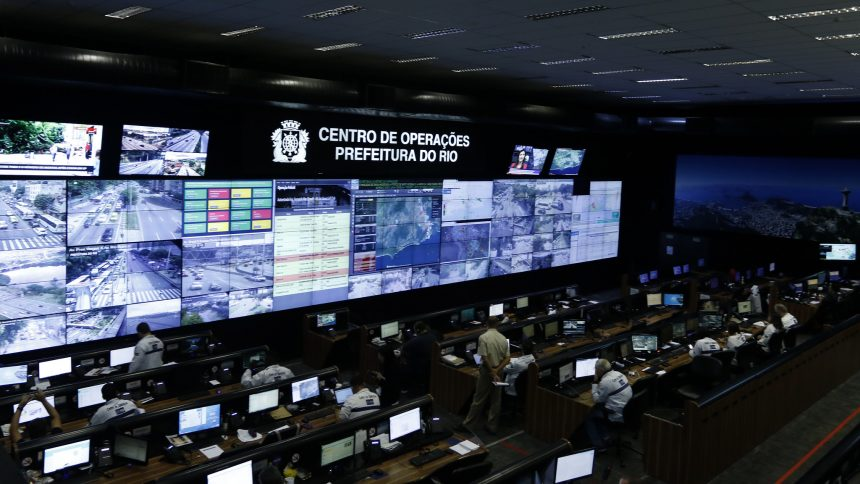
\includegraphics[width=0.9\linewidth]{images/46627458084_451cf87027_k.jpg}}
\caption{Sala central do Centro de Operações do Rio}
\label{fig:cor}
\end{figure}

\section{Objetivo}

Com base em diversas pesquisas sobre o problema das inundações urbanas utilizando diferentes Redes Neurais Convolucionais (CNN, do inglês \acrlong{cnn}),
apresentadas na Seção \ref{sec:trabalhos_alagamento},
a presente dissertação visa desenvolver uma abordagem inicial utilizando \acrshort{cnn}s com aprendizado por transferência (\textit{transfer learning}), treinadas em um conjunto de dados original,
para não apenas facilitar o monitoramento e classificação das milhares de câmeras na cidade do Rio de Janeiro pelo \acrshort{cor}.

Portanto, esta pesquisa foi estruturada em quatro etapas principais: (i) aquisição e preparação dos dados, (ii) seleção das arquiteturas de redes neurais, (iii) treinamento e validação dos modelos, e (iv) avaliação do desempenho e análise dos resultados.

Os dados foram obtidos por meio de câmeras do \acrshort{cor}, enquanto a escolha das arquiteturas foi embasada em uma revisão criteriosa da literatura referente ao reconhecimento e classificação de alagamentos.

O treinamento e a validação foram conduzidos inicialmente por meio de validação simples, com o intuito de identificar o modelo de melhor desempenho. Posteriormente, esse modelo selecionado foi submetido a uma validação cruzada, proporcionando uma avaliação mais robusta e confiável dos seus resultados.

Finalmente, o desempenho do modelo foi comparado com resultados obtidos em outros conjuntos de dados, visando avaliar sua capacidade de generalização.

A seção seguinte apresenta uma descrição dos capítulos que abordam cada uma dessas etapas de forma aprofundada.

%Todos os modelos foram treinados em conjunto de dados original formado por imagens do circuito de câmeras do Centro de Operações do Rio.
%Todas as câmeras neste conjunto de dados são fixas, de forma que não há nenhuma modificação na paisagem ao longo do dia.

\section{Organização do Texto}\label{Organização do texto}

O capítulo \ref{cap:fundamentação} explica brevemente os conceitos mais importantes para o desenvolvimento deste trabalho, começando por técnicas de processamento de imagem e finalizando na abordagem dos fundamentos de redes neurais.

O capítulo \ref{cap:trabalhos} considera alguns trabalhos relevantes para o problema de classificação do estado de alagamento em regiões urbanas nos últimos 5 anos.
Ao final, algumas características das tecnologias utilizadas em cada artigo, assim como as deste trabalho, são comparadas em uma tabela.

O capítulo \ref{cap:metodologia} descreve a metodologia usada na execução deste trabalho,
explicando a criação do conjunto de dados, a escolha das arquiteturas de \acrshort{cnn}s inicialmente empregadas e as métricas utilizadas para a comparação dos resultados.

O capítulo \ref{cap:resultados} apresenta e discute os resultados do treinamento das diferentes arquiteturas comparadas.
O modelo com melhor performance é mais detalhadamente avaliado após a inclusão de alterações no pré-processamento e uso de diferentes conjuntos de dados de entrada.

O capítulo \ref{cap:conclusoes} sumariza as contribuições e limitações deste trabalho, apresentando conclusões relacionadas aos seus resultados.
Também discute possíveis pontos para melhorias futuras em prosseguimentos da linha de pesquisa.

No Apêndice \ref{apendA} estão citadas os códigos das câmeras do COR usadas e os números de imagens de cada classe delas armazenadas no conjuntos de dados inicial da pesquisa.

\section{Contribuições e legados concretos desta dissertação}\label{Contribuições}

Até o momento com os resultados deste trabalho foram publicados no IEEE \cite{goncalves2024} contribuindo, também, com a disponibilização dos três conjuntos de dados (treino, validação e teste)
correspondentes a organização que se fez nas diversas etapas desta dissertação e os programas de computador (fontes e executáveis) desenvolvidos. 
Esses se encontram publicamente disponíveis em \href{https://doi.org/10.5281/zenodo.15670835}{10.5281/zenodo.15670835}.

%\pagestyle{ruledheader}
%\include{capitulos/cap2}  %inclui novo capítulo

%\pagestyle{ruledheader} %inclui novo capítulo
%\include{capitulos/cap2}
\pagestyle{ruledheader}
\chapter{Fundamentação Teórica}\label{cap:fundamentação}

Este capítulo explica de forma breve os conceitos necessários para entender todas as ferramentas usadas no capítulo \ref{cap:metodologia}. 
Para isso, o capítulo é dividido em duas sessões, onde a primeira se baseia em conceitos de processamento de imagem. Já a segunda sessão é dedicada exclusivamente para redes neurais convolucionais e as arquiteturas utilizadas.

\section{Técnicas de Processamento de Imagens}

Este trabalho foi desenvolvido em Python, utilizando a biblioteca \textit{Pillow} para manipular imagens.
As equações que definem as conversões entre espaços são descritas de acordo com a documentação do \textit{Pillow}\cite{clark2015pillow}.
\subsection{Espaço de Cores}
Uma imagem colorida é composta por uma ou mais bandas. 
Usualmente, uma imagem digital em cores é composta por três bandas monocromáticas, onde cada banda armazena uma informação diferente da imagem colorida no pixel p(m,n) da banda. 

Cada banda (ou canal), de largura M pixels e altura N pixels, pode ser considerada como um plano onde um pixel está relacionado a um par de coordenadas inteiras p(m,n) pertencente à banda. 
O valor armazenado na posição m,n no plano indica a intensidade da banda na imagem naquele ponto, usualmente com 256 possíveis valores diferentes de serem armazenados em um byte. 
Onde 0 é a intensidade mais escura e 255 a intensidade mais clara \cite{jaelim, shapiro}.

Existem espaços diferentes de representação de cores, sendo o mais comum o RGB CIE (sigla para \textit{Commission internationale de l'éclairage}) de 1931, 
ou simplesmente RGB (do inglês \textit{Red, Green and Blue}). 
Neste espaço cada cor aparece em seu componente espectral primário correspondente a essas cores, de modo que cada banda armazena unicamente a informação da intensidade do vermelho, verde e azul respectivamente \cite{gonzalez, jaelim}. 
O espaço de cores XYZ-CIE 1931 (XYZ) foi projetado para representar todas as cores visíveis, mesmo as que não são representáveis no RGB. 
As componentes X e Z são elementos sem visibilidade aos olhos humanos, portanto, não existem na práticas como cores \cite{ohta}. 
O componente Y representa a luminância ou a melhor representação monocromática possível da cena originalmente colorida.
% -----------------------

\subsection{Conversões entre RGB e YCbCr}
% https://github.com/python-pillow/Pillow/blob/61a35f94cf8a217db3e67d32db943b05e593e781/src/libImaging/ConvertYCbCr.c#L17-L21

Nestas conversões não há nenhum tipo de alteração nos valores dos pixels no espaço de cor original antes de convertê-los para pixels no espaço de cor desejado.
As equações \ref{eqn:ycrcb_y}, \ref{eqn:ycrcb_cb} e \ref{eqn:ycrcb_cr} mostram a conversão do espaço RGB para YCbCr.
Já as equações \ref{eqn:rgb_r}, \ref{eqn:rgb_g} e \ref{eqn:rgb_b} mostram a conversão do espaço YCbCr para RGB.

\begin{equation}
    \label{eqn:ycrcb_y}
    Y \xleftarrow{} R \cdot 0,29900 + G \cdot 0,58700 + B \cdot 0,11400
\end{equation}
\begin{equation}
    \label{eqn:ycrcb_cb}
    Cb \xleftarrow{} R \cdot -0,16874 + G \cdot -0,33126 + B \cdot 0,50000 + 128
\end{equation}
\begin{equation}
    \label{eqn:ycrcb_cr}
    Cr \xleftarrow{} R \cdot 0,50000 + G \cdot -0,41869 + B \cdot - 0,08131 + 128
\end{equation}

\begin{equation}
    \label{eqn:rgb_r}
    R \xleftarrow{} Y + (Cr - 128) \cdot 1.40200
\end{equation}
\begin{equation}
    \label{eqn:rgb_g}
    G \xleftarrow{} Y + (Cb - 128) \cdot -0,34414 + (Cr - 128) \cdot -0,71414
\end{equation}
\begin{equation}
    \label{eqn:rgb_b}
    B \xleftarrow{} Y + (Cb - 128) \cdot 1,77200
\end{equation}

% \begin{equation}
%     \label{eqn:ycrcb_y}
%     Y \xleftarrow{} 0,299\cdot R + 0,597\cdot G + 0,114\cdot B
% \end{equation}
% \begin{equation}
%     \label{eqn:ycrcb_cb}
%     Cb \xleftarrow{} (B-Y)\cdot 0,564 + delta
% \end{equation}
% \begin{equation}
%     \label{eqn:ycrcb_cr}
%     Cr \xleftarrow{} (R-Y)\cdot 0,713 + delta
% \end{equation}
% onde
% \begin{equation}
%     \label{eqn:ycrcb_delta}
%     delta \xleftarrow{}
%     \begin{cases}
%     128 & \text{para imagens de 8 bits por canal}\\
%     32768 & \text{para imagens de 16 bits por canal}\\
%     0,5 & \text{para imagens normalizadas entre 0 e 1}
%     \end{cases}
% \end{equation}

% -----------------------
\subsection{Transformações de Intensidade no Domínio Espacial}

As transformações de intensidade são funções matemáticas no domínio espacial da imagem, que operam diretamente no valor dos pixels da imagem de entrada \cite{gonzalez}.
Essas funções podem ser representadas pela expressão:
\begin{equation}
    \label{eqn:intensitytransformation}
    g(x,y) = T\left [ f(x,y) \right ]
\end{equation}
onde \textit{f(x,y)} é a imagem de entrada, \textit{g(x,y)} é a imagem de saída e \textit{T} é uma função definida sobre um ponto \textit{x,y} ou sua vizinhança.

Uma das transformações de intensidade mais simples é a transformação linear, onde os valores de intensidade de um canal são multiplicados por uma constante, como representado pela equação:
\begin{equation}
    \label{eqn:linearintensitytransformation}
    i^{'} = \alpha \times i
\end{equation}

Através da equação \ref{eqn:linearintensitytransformation}, a intensidade \textit{i} de um pixel é multiplicada pelo fator de escala $\alpha$, resultando na nova intensidade  $i^{'}$.

% -----------------------
\subsection{Filtragem por convolução}

Também chamados de máscaras ou kernels, filtros são matrizes de tamanho $m \times n$ aplicadas sobre uma imagem através de multiplicações pelos valores das máscaras e somas, cujos resultados serão os valores da imagem processada.
Suas dimensões e valores que a compõem variam dependendo da característica a ser extraída de cada vizinhança $m \times n$ da imagem, como detecção de bordas ou texturas \cite{shapiro}.
% ----------------------------------------------------------
\section{Redes Neurais Convolucionais}

As redes neurais convolucionais, ou \acrshort{cnn}s, são uma classe especial de redes neurais artificiais que se especializam em processar dados com uma topologia em matrizes \cite{Goodfellow-et-al-2016}. 

Inspiradas pela organização do córtex visual dos mamíferos \cite{hubel1962}, as \acrshort{cnn}s são projetadas para 
%capturar hierarquicamente características espaciais e visuais em imagens, permitindo a extração e o aprendizado de feições cada vez mais abstratas e de alto nível. Nesta seção, abordaremos os fundamentos das CNNs, incluindo suas principais camadas, funcionamento e aplicações em análise de imagens.
extrair características locais que dependem de uma pequena vizinhança na imagem, onde estas pequenas características podem ser usadas por outras camadas para detectar características de maior ordem e extrair informações sobre a imagem \cite{book:Bishop}. 

\acrshort{cnn}s são usadas principalmente para tarefas que trabalham em imagens, como reconhecimento de objetos, segmentação de imagens e detecção de padrões complexos de dados visuais.

O aprendizado de características locais permite que a \acrshort{cnn} reconheça esses padrões em qualquer outro local da imagem,  tornando-a invariante a translação. A utilização de características de uma camada por camadas sucessivas permite que a \acrshort{cnn} aprenda padrões espaciais hierárquicos \cite{book:Chollet}.

% -----------------------
\subsection{Arquitetura de uma Rede Neural Convolucional}

A arquitetura básica de uma \acrshort{cnn} inclui três tipos principais de camadas: convolucional, de pooling e totalmente conectada. 
Uma \acrshort{cnn} típica é formada por pares de camadas de convolução e de pooling empilhadas, que ao final são ligadas a uma camada totalmente conectada.
A Figura \ref{fig:cnn_arch} mostra uma arquitetura genérica de \acrshort{cnn}. 

\begin{figure}[htb]
\centerline{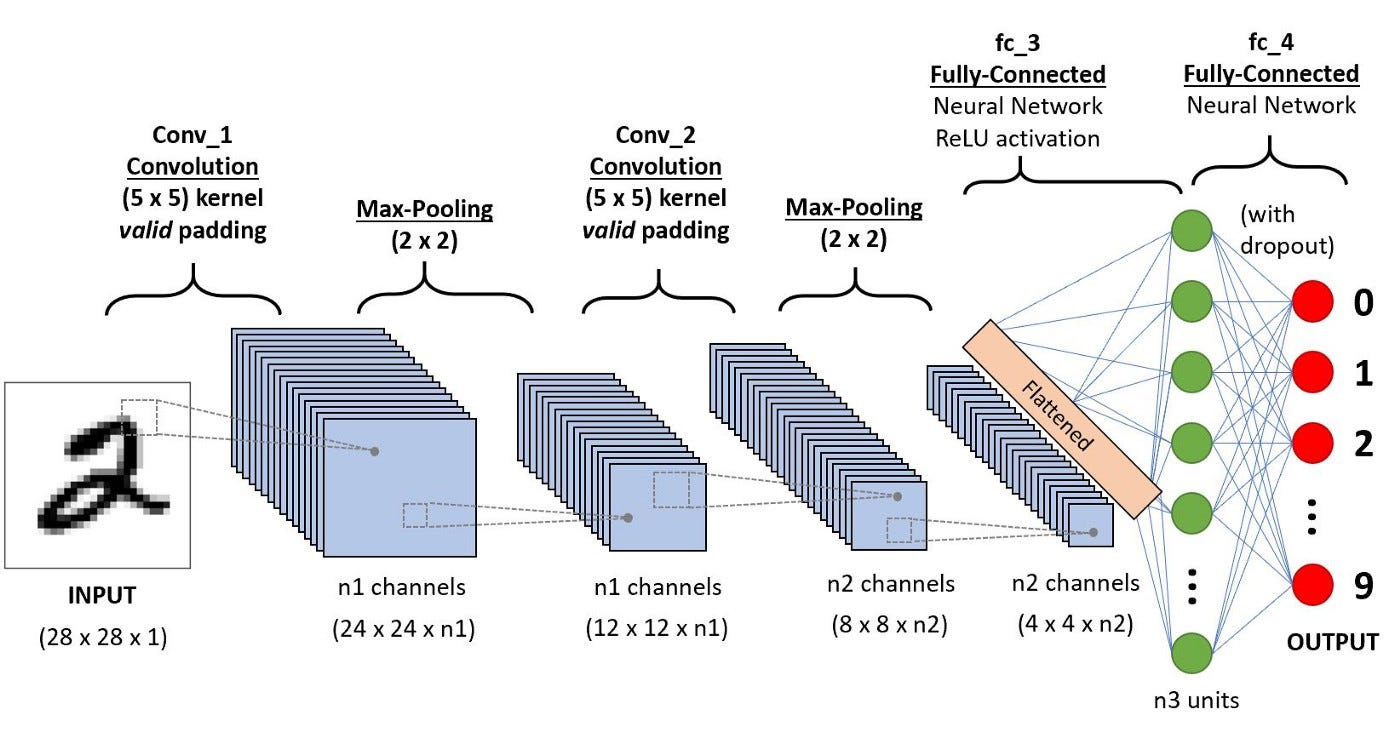
\includegraphics[width=1\linewidth]{images/cnn_placeholder.jpg}}
\caption{Arquitetura de uma \acrshort{cnn} genérica.}
\label{fig:cnn_arch}
\end{figure}

% -----------------------
\subsubsection{Camada Convolucional}

A camada convolucional é o núcleo de uma \acrshort{cnn} e é responsável pela extração de características. 
Para isso pesos na forma de kernels, ou filtros da Análise de Imagem tradicional, 
são aplicados sobre a imagem, onde são escorregados e multiplicados pelos valores dos pixels da imagem de entrada e somados resultando em um pixel para cada kernel, 
usando uma quantidade definida de passos. Esse processo gera os mapas de características, onde cada mapa representa a resposta de um filtro específico a uma região da imagem de entrada. 
Essa camada detecta padrões locais como bordas, texturas ou formas, (de acordo com o kernel usado) que podem ser usados para extrair informações de padrões mais complexos conforme a rede se aprofunda.

A operação de convolução S entre um filtro I e uma entrada K pode ser representada como:

\begin{equation}
    \label{eqn:convolution}
    S(x,y) = \sum_{m}\sum_{n}I(x+m,y+n)K(m,n)
\end{equation}
onde S(x,y) é o mapa de características gerado (saida), I(x,y) representa a entrada local (imagem original) e K(m,n) o kernel aplicado.
% -----------------------
\subsubsection{Camada de Pooling}

%A camada de pooling é utilizada para reduzir a dimensionalidade dos mapas de características, preservando as informações mais relevantes e diminuindo o custo computacional da rede. As operações de pooling ajudam a tornar a rede menos sensível a pequenas variações e deslocamentos na imagem, além de promover uma forma de regularização que reduz o risco de overfitting.

A camada de pooling altera a saída da camada convolucional com um resumo estatístico de uma vizinhança, melhorando a eficiência computacional da rede pela diminuição da dimensionalidade da saída e ajudando a tornar a saída menos variante a translações da entrada.
Este resumo estatístico pode ser feito com diferentes operações. Por exemplo a arquitetura VGG19 \cite{vgg} utiliza \textit{max pooling}, onde a saída é o maior valor na vizinhança analisada. A operação \textit{average pooling} é utilizada no InceptionV3 \cite{inceptionv3}, onde a média da vizinhança é calculada.


% -----------------------
\subsubsection{Camada Totalmente Conectada}

Estas são geralmente as últimas camadas em uma \acrshort{cnn}, sendo responsáveis pela combinação das características extraídas nas camadas anteriores para realizar a classificação final. 
Nesta camada, todos os neurônios estão conectados a cada unidade da camada anterior, como um perceptron multicamadas comum \cite{MURTAGH1991183}. 
O seu aprendizado é feito por um algoritmo de retro-propagação de erro \cite{Rumelhart1986LearningRB}.
% -----------------------
\subsection{Processo de Treinamento de uma CNN}

O treinamento de uma \acrshort{cnn} é realizado por meio de aprendizado supervisionado, onde o modelo ajusta os pesos e vieses das camadas convolucionais (totalmente conectadas) para minimizar a diferença entre as previsões e os rótulos verdadeiros.

A função de perda, que calcula o erro da rede, é derivada e propagada para ajustar os pesos de forma iterativa. 
Este trabalho utilizou a Entropia Cruzada como função de perda, que é definida por:

% Retirado de Goodfellow
\begin{equation}
    \label{eqn:crossentropy}
    H(P,Q) = -E_{P}[log Q]
\end{equation}
onde H(P,Q) é a entropia cruzada da distribuição Q em relação a distribuição P, sendo a distribuição Q o resultado da \acrshort{cnn} e a distribuição P a distribuição de treinamento \cite{mao2023}. 
$E_{P}[.]$ é o valor esperado em relação a distribuição P.

Para minimizar a função de perda, foi usada a descida de gradiente estocástica (\acrshort{sgd}, do inglês \acrlong{sgd}) \cite{ruder2016}. Enquanto a descida de gradiente padrão calcula o gradiente utilizando todo o conjunto de dados, o \acrshort{sgd} utiliza amostras de dados para o cálculo do gradiente na iteração atual.
Dessa forma, a \acrshort{sgd} altera o valor dos parâmetros da seguinte forma:
%Retirado de Bishop
\begin{equation}
    \label{eqn:sgd}
    \omega^{\tau+1} = \omega{\tau} - \eta\Delta{E}
\end{equation}
onde $\omega$ é o peso sendo usado, $\tau$ é o número da iteração, $\eta$ é a taxa de aprendizado e $\Delta{E}$ é o gradiente do erro.

% -----------------------
\subsection{Aprendizado por Transferência}
% IBM, Wikipedia e UFSC referenciam por 'Aprendizado por transferência', AWS e UFRJ referenciam por 'Transferência por aprendizado'
Uma possibilidade importante nas \acrshort{cnn}s é o uso de redes pré-treinadas e aprendizado por transferência (\textit{transfer learning}), 
onde os pesos dos modelos pré-treinados em grandes conjuntos de dados são aproveitados e ajustados para problemas específicos com menos dados, 
reduzindo o tempo de treinamento e melhorando a precisão em aplicações com conjuntos de dados menores. 
Neste trabalho, o aprendizado por transferência baseado no IMAGENET \cite{deng2009imagenet} foi aplicado em todos os modelos avaliados, alterando sua última camada para uma classificação binária.
% -----------------------
\subsection{Visual Geometry Group (VGG)}
A \acrshort{vgg} é uma família de \acrshort{cnn}s que possuem arquiteturas simples. 
Propostas por \cite{vgg}, as \acrshort{vgg}s são compostas por blocos uniformes empilhados com duas camadas convolucionais e uma camada de \textit{pooling}. 
As camadas de \textit{pooling} têm tamanho 2x2 reduzindo a dimensionalidade da convolução pela metade. 

Já as camadas convolucionais compartilham do mesmo tamanho de filtro, sendo estes 3x3. Além disso, cada bloco dobra a quantidade de filtros de suas camadas convolucionais em relação ao bloco anterior. Por exemplo, o primeiro bloco de uma rede \acrshort{vgg} possui 64 filtros 3x3 em suas camada convolucionais, enquanto o segundo bloco possui 128 filtros 3x3.

Este trabalho utilizou a \acrshort{vgg}-19, que indica a existência de 19 camadas de aprendizado, contando não só as camadas convolucionais como as camadas completamente conectadas.
% -----------------------
\subsection{Inception}

Diferente do \acrshort{vgg}, a família \textit{Inception}\cite{inception} de \acrshort{cnn}s utiliza o empilhamento de módulos Inception, onde convoluções de diferentes tamanhos são realizadas no mesmo módulo, especificamente convoluções de 1x1, 3x3 e 5x5. Ao final, tais convoluções são concatenadas junto ao \textit{pooling} da própria entrada, gerando a saída do módulo. 

O \textit{InceptionV3}\cite{inceptionv3} fatoriza convoluções maiores em uma sequência de convoluções menores. A convolução 5x5, por exemplo, é substituída por duas convoluções 3x3, diminuindo a quantidade de parâmetros mas mantendo a expressividade das características extraídas.

Outra modificação implementada no \textit{InceptionV3} foi a utilização do \textit{label smoothing}, onde a confiança do modelo é reduzida para evitar \textit{overfitting}. Isso é feito alterando a probabilidade esperada de cada classe:

\begin{equation}
    \label{eqn:labelsmoothing}
     q(k) = (1-\epsilon )\delta _{k,j}+\frac{\epsilon }{K}
\end{equation}

Onde \textit{j} é a classe correta, \textit{k} é a classe sendo avaliada, $\delta_{k,j}$ é o \textit{Delta de Dirac}, que se torna 1 quando \textit{k = j} e 0 em qualquer outro caso, $\epsilon$ é uma probabilidade de incerteza do modelo, e \textit{K} é o número de classes. Portanto, o \textit{label smoothing} retira da probabilidade \textit{1} da classe correta uma incerteza $\epsilon$ e a distribui igualmente entre as outras \textit{K} classes do problema.
% -----------------------
\subsection{DenseNet}

A característica de maior importância da \textit{DenseNet}\cite{densenet} é que sua arquitetura é baseada em blocos densos, 
que são compostos por camadas convolucionais onde sua entrada recebe a saída de todas as camadas convolucionais anteriores a ela. 
Os blocos densos são ligados por camadas de transição, compostas por uma camada de convolução 1x1 e uma camada de \textit{average pooling} 2x2. 
A arquitetura de uma \textit{DenseNet} simples pode ser vista na Figura \ref{fig:densenet_arch} \cite{densenet}.

\begin{figure}[htb]
\centerline{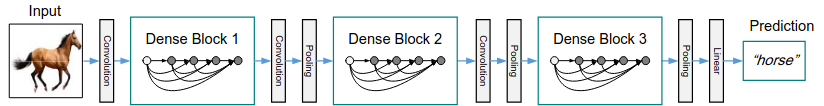
\includegraphics[width=1\linewidth]{images/densenet.png}}
\caption{Arquitetura de uma \textit{DenseNet} genérica\cite{densenet}.}
\label{fig:densenet_arch}
\end{figure}

% -----------------------
\subsection{MobileNet}
A família \textit{MobileNet} de redes neurais foi desenvolvida para utilização por aplicações móveis ou embarcadas \cite{mobilenet}, 
posuindo arquiteturas mais simples e leves em comparação a outras redes neurais profundas, 
mas continuam a oferecer boa performance. Sua maior distinção de outras \acrshort{cnn}s é a introdução de convoluções separáveis em profundidade, que substituem as convoluções tradicionais.

As convoluções separáveis em profundidades fatorizam uma convolução comum em uma convolução em profundidade e uma convolução 1$\times$1, também chamada de convolução pontual. Isso significa que na convolução em profundidade, em vez de aplicar um filtro que abrange todos os canais da janela a qual está realizando a convolução, será aplicada um filtro por canal, onde a saída de cada canal é combinada pela convolução pontual, reduzindo o custo computacional envolvido na convolução.

Além disso, a arquitetura também possui dois hiperparâmetros globais, um multiplicador de largura $\alpha$ e um multiplicador de resolução $\rho$, que servem para reduzir o custo computacional da rede. O hiperparâmetro $\alpha$ serve para afinar a rede neural em cada camada por um fator $\alpha$, aplicado tanto no número de canais de entrada quanto de canais de saída. Já o hiperparâmetreo $\rho$ é aplicado na imagem de entrada e nas representações internas de cada camada, multiplicando-os por $\rho$.

A arquitetura \textit{MobileNetV2}\cite{mobilenetv2} introduz blocos inversos residuais na arquitetura da rede. Este bloco aumenta a dimensionalidade da entrada através de um conjunto de convoluções 1$\times$ 1 e aplica uma convolução em profundidade em seguida, para capturar informações em cada canal expandido. Ao final, uma convolução 1x1 é aplicada para reduzir os canal de volta ao tamanho original.

% -----------------------
\subsection{Visual Transformer (ViT)}
A arquitetura \textit{Visual Transformer}\cite{vit} aplica o conceito de \textit{transformers}\cite{transformer2017} 
utilizados em processamento de linguagem natural para tarefas de classificação de imagens, como alternativa às \acrshort{cnn}s. 
A arquitetura em si é relativamente simples, composta um \textit{transformer enconder}, sem a utilização de um \textit{transformer decoder}, 
que fornece sua saída a um perceptron multicamadas simples (\acrshort{mlp}, do inglês \acrlong{mlp}), sendo este o responsável pela classificação. 
Apesar de simples, nos processos necessários para enviar a imagem para o \textit{transformer} é onde a complexidade da arquitetura aparece.

A Figura \ref{fig:vit_arch} \cite{vit}, mostra a arquitetura de um \acrshort{vit}. 
Diferente de uma \acrshort{cnn} comum, a imagem é dividida em blocos de tamanho fixo denominados \textit{patches}. 
Esses \textit{patches} são transformados em vetores e linearizados. 
Para convertê-los ao espaço de características do modelo, os \textit{patches} passam por um \textit{embedding}, através de uma projeção em um espaço de dimensão fixa. 
Antes de enviar a sequência de \textit{embeddings} ao \textit{transformer}, 
é necessário adicionar um \textit{token} de posicionamento para informar à rede sobre a posição de cada \textit{patch} na imagem original. 
Além desses \textit{token}s, um \textit{token} adicional \textit{class} é colocado no início da sequência, que receberá a saída do processamento realizado pelo \textit{transformer}.

\begin{figure}[htb]
\centerline{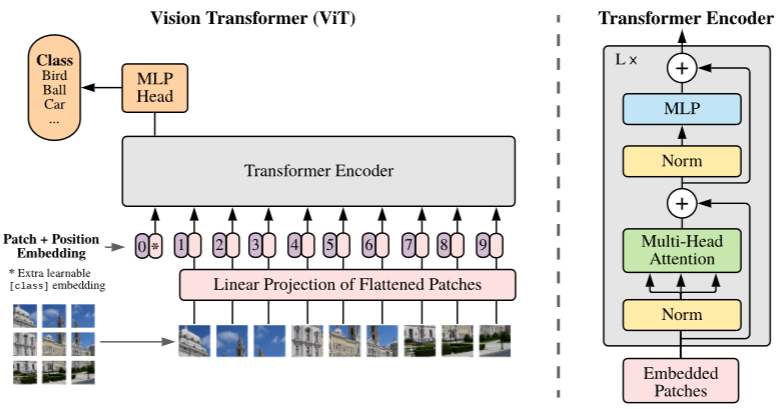
\includegraphics[width=1\linewidth]{images/visual transformer.png}}
\caption{Arquitetura de um \textit{Visual Transformer}\cite{vit}.}
\label{fig:vit_arch}
\end{figure}

O \textit{Transformer} é uma sequência de pares de camadas alternadas, o tamanho dessa sequência de camadas define a profundidade do modelo. 
O primeiro par de camadas consiste em uma camada de normalização, transformando os valores de todos os elementos da sequência para limites predefinidos, e uma camada de \textit{Multi-Headed Self-Attention}, onde é computada uma soma ponderada de entre cada par de elemento do \textit{patch}.
O segundo par de camadas possui uma camada de normalização e uma camada de \acrshort{mlp}, para processar cada elemento do \textit{patch}.

O processamento final do \textit{transformer} é enviado para um \acrshort{mlp} final denominado \textit{MLP Head}, responsável por receber o \textit{token} \textit{class} que representa as informações da imagem aprendidas no \textit{transformer}, e utilizá-lo para gerar a classificação final da imagem.

\pagestyle{ruledheader}
\chapter{Trabalhos Relacionados}\label{cap:trabalhos}
Diversos estudos vêm sendo realizados na área de classificação e detecção de inundações, utilizando tanto algoritmos tradicionais de aprendizado de máquina quanto redes neurais profundas. Tais pesquisas empregam diferentes fontes de dados, incluindo imagens capturadas por satélites, imagens provenientes de câmeras fixas e, ainda, dados numéricos obtidos a partir de instrumentos de medição, como pluviômetros, entre outros.

Neste capítulo, inicialmente serão apresentados trabalhos que empregaram algoritmos de aprendizado de máquina para prever eventos de alagamento. Em seguida, serão brevemente descritos estudos que utilizaram imagens de satélite para a análise de áreas alagadas, incluindo uma seção dedicada à aplicação de arquiteturas do tipo \textit{U-Net} para segmentação e classificação dessas imagens.

Por fim, a última seção será dedicada a pesquisas cujo foco principal é a classificação de imagens relacionadas a alagamentos urbanos. Devido ao foco desta dissertação estar centrado na classificação de imagens capturadas por sistemas de câmeras urbanas, essa seção será discutida com maior profundidade em relação às anteriores.

Para facilitar a compreensão da evolução do campo, os trabalhos apresentados em cada seção serão organizados em ordem cronológica, iniciando pelos mais antigos.
% ----------------------------------------------------------
\section{Aprendizado de Máquina}

Utilizando dados disponibilizados pelo Departamento Meteorológico de Bangladesh (\textit{Bangladesh Meteorological Department}) e pelo Conselho de Desenvolvimento Hídrico de Bangladesh (\textit{Bangladesh Water Development Board}), Toufique \textit{et al.} \cite{toufique2024} treinaram quatro algoritmos de aprendizado de máquina para a predição de inundações na região. Entre os modelos avaliados, o \textit{Random Forest} \cite{randomforest} apresentou o melhor desempenho, alcançando uma acurácia de 85,6\%.

Jamunadevi \textit{et al.} \cite{jamunadevi2024} propuseram uma abordagem híbrida que combinou uma rede neural recorrente do tipo memória de curto e longo prazo (LSTM) \cite{lstm} com uma rede neural convolucional (\acrshort{cnn}), visando a previsão de alagamentos ao longo de um período de um ano no estado de Tamil Nadu, Índia. Os dados utilizados para treinamento englobaram variáveis meteorológicas e ambientais, tais como temperatura, umidade, precipitação, velocidade do vento, radiação solar e evapotranspiração. O modelo desenvolvido obteve uma acurácia de 97,4\% na previsão dos eventos de alagamento ocorridos em 2024.

Vimala \textit{et al.} \cite{vimala2024} empregaram um conjunto de 22 indicadores ambientais para realizar a predição de alagamentos, utilizando seis algoritmos de aprendizado supervisionado, incluindo o \textit{Random Forest}. Entre os modelos testados, a Regressão Logística \cite{cramerlogisticregression} foi o que apresentou o melhor desempenho, com uma acurácia de 99,85\%, enquanto o \textit{Random Forest} atingiu uma acurácia de 89,37\%.

Shah \textit{et al.} \cite{shah2024} utilizaram os algoritmos \textit{Random Forest} e \textit{XGBoost} \cite{chenxgboost} para gerar um mapa de suscetibilidade a inundações da cidade de Chennai, também no estado de Tamil Nadu. Os autores empregaram seis métricas provenientes de três fontes distintas para treinar os modelos, nos quais o \textit{XGBoost} apresentou a melhor acurácia, alcançando 70\%.

% ----------------------------------------------------------
\section{Imagens de Satélite}

Kool \textit{et al.} \cite{KOOL2022102766} classificaram o estado de inundação sazonal de um pântano em Mara na Tanzânia. 
Para isso, treinaram um \textit{Random Forest} sazonalmente em conjuntos de imagens do satélite Sentinel-2 \cite{sentinel2}, obtendo acurácia de 98,6\%.

Siddique \textit{et al.} \cite{siddique2023} propuseram uma abordagem integrada utilizando \textit{Random Forest}, \acrfull{knn}\cite{knn1967} e \textit{k-means}\cite{kmeans2023} 
para classificar imagens do satélite Sentinel-1 \cite{sentinel1} do estado da Índia de Uttar Pradesh. Obtendo acurácia de 97,0\% para a cidade de Basti e 93,8\% para a cidade de Ayodhya, ambas no estado de Uttar Pradesh.

Reddy e Vimal \cite{reddy2024} classificaram 400 imagens de satélites, obtendo resultados de 92,72\% de acurácia com análise discriminante linear \cite{lda} e 95,05\% com AlexNet \cite{alexnet}.

Cao \textit{et al.} \cite{cao2024} utilizaram uma \acrshort{cnn} simples, proposta pelos autores, onde a saída da camada completamente conectada alimenta um 
classificador de Máquina de Vetores de Suporte (\acrshort{svm}, do inglês \acrlong{svm}) \cite{svm} para classificar o pântano de Qilihai, na China. Obtiveram acurácia de 90,3\% no conjunto de dados,
que foi montado através de imagens do Sentinel-1 e Sentinel-2.

Myin e Thein \cite{myin2024} aplicaram um \textit{Random Forest} em 1000 imagens do Sentinel-1 da região de Bago, em Myanmar, com acurácia de 93,18\%. 

Huang \textit{et al.} \cite{huang2024} projetaram um modelo chamado \textit{WaterDetectionNet} (WDNet) para mapear alagamentos, 
usando imagens de radar de abertura sintética \cite{sar} do Sentinel-1 sobre lago de Poyang, na China. O modelo WDNet com módulo de atenção própria atingiu acurácia de 98,7\%.

Bouchelkia \textit{et al.} \cite{bouchelkia2024} propuseram um abordagem para dectectar diferenças em terrenos pós-inundações, 
com pares de imagens do Sentinel-2 antes e depois da ocorrência de inundações na cidade de Derna na Líbia. 
A arquitetura de rede neural profunda \cite{dnn} proposta pelos autores obteve área sobre união de 95,8\%.

Sudiana \textit{et al.} \cite{sudiana2025} classificaram imagens do Sentinel-1 de áreas urbanas em Jacarta, capital da Indonésia, utilizando uma \textit{3D-}\acrshort{cnn} \cite{3dcnn}.
Conseguiram acurácia de 71,8\% com 20 imagens de satélite.

\subsection{U-Net}
Com o objetivo de segmentar e classificar imagens de alagamento de diferentes fontes, Ahmed \textit{et al.} \cite{ahmed2024} compararam diferentes arquiteturas para esses trabalhos: 
\textit{DeepLabv3}\cite{chen2017deeplabsemanticimagesegmentation}; \textit{MaskRCNN} \cite{maskrcnn}; e \textit{U-Net} \cite{unet}.
O DeepLabv3 obteve interseção sobre união \cite{iou2019} médio de 0,95, em comparação com 0,93 do \textit{MaskRCNN} e 0,94 do \textit{U-Net}.

Alhady \textit{et al.} \cite{alhady2024} compararam a performance do \textit{U-Net} em imagens do Sentinel-2 com diferentes métodos de índice de água \cite{waterindex}, onde a utilização do
\textit{Modified Normalized Difference Water Index} \cite{mndwi} obteve a melhor performance, com área sobre união de 97,71\%/.

Chandram \textit{et al.} \cite{chandran2024} propuseram um sistema de detecção de alagamentos baseado no \text{U-Net} com área sobre união de 0,85.

Pech-May \textit{et al.} \cite{pech-may2024} classificaram imagens do Sentinel-1 do estado mexicano de Tabasco, utilizando o \textit{U-Net}. Os autores compararam a acurácia de área sobre união
treinando em diferentes épocas, onde o modelo treinado em 200 épocas foi o melhor, com acurácia de 94,31\% e área sobre união de 0,730.
% ----------------------------------------------------------
\section{Alagamento em áreas urbanas}\label{sec:trabalhos_alagamento}
%A Hybrid Machine Learning Approach for Classifying Aerial Images of Flood-Hit Areas
Akshya e Priyadarsini \cite{akshya2019} utilizaram imagens aéreas de áreas alagadas na Índia para classificar o grau de severidade de alagamentos. 
Inicialmente, é realizada a extração de características utilizando \acrfull{bovw}. Depois uma clusterização com \textit{k-means}. 
Na classificação eles usaram uma abordagem híbrida, feita através de uma \acrshort{svm}. 
Usando um conjunto de dados de 200 imagens, sendo 100 para cada classe, a abordagem conseguiu acurácia média de 92\%.
Apesar da abordagem interessante de utilizar \Acrshort{bovw} para classificação com aprendizado de máquina clássico, os autores somente avaliaram \acrshort{svm} com diferentes \textit{kernels},
sem comparar com outros algoritmos de aprendizado de máquina. Além disso, o modelo não só foi testado em somente um conjunto de dados, como o conjunto de dados usado não foi disponibilizado.

%Detecting floodwater on roadways from image data with handcrafted features and deep transfer learning
Sazara \textit{et al.} \cite{sazara2019} abordaram o problema de classificação de inundação (ou não em imagens) utilizando a saída de um extrator de características para treinar modelos de aprendizado de máquina diferentes. 
Para extração de características foram avaliados Padrões Locais Binários (LBP) , Histograma de Gradientes Orientados (HOG) e uma rede neural \acrshort{vgg}-16. 
Os modelos de aprendizado de máquina treinados nas características extraídas foram a Regressão Logística, k-NN, e uma Árvore de Decisão. 
A combinação que forneceu melhores resultados, com precisão de 0,94 e revocação de 0,97 , 
foi o uso da \acrshort{vgg}-16 como extrator de características e a Regressão Logística como classificador. 
O conjunto de dados utilizado consistiu de 253 imagens de alagamento e 238 sem alagamento foi disponibilizado e foi usado para comparação do melhor modelo desta pesquisa, na Seção \ref{sec:resultados_outros}.
Entretanto, os autores não avaliram o modelo em outros conjuntos de dados.

%Flood Detection in Social Media Images using Visual Features and Metadata
Jony \textit{et al.} \cite{jony2019} classificaram binariamente alagamentos em imagens retiradas de redes sociais. 
Para isso, utilizaram três diferentes \acrshort{cnn}s para extração de características com uma simples rede neural para classificação binária do problema, usando duas abordagens, 
sobre o conjunto de dados do \textit{Disaster Image Retrieval from Social Media} 2017\cite{dirsm2017}. 
A primeira abordagem utilizou InceptionV3 e Xception como extratores, enquanto a segunda abordagem utilizou \acrshort{vgg}-16 como extrator. 
Os resultados mostraram que realizar uma média dos resultados de cada classe entre as duas abordagens gerou melhor acurácia que usar cada abordagem unicamente. 
As abordagens em conjunto, a primeira abordagem e segunda abordagem tiveram acurácia de 93\% , 92,8\% e 90,6\% respectivamente.
Este trabalho utilizou o conjunto de dados do desafio \textit{MediaEval 2017} e comparou seus resultados com outros métodos apresentados no mesmo desafio, obtendo resultados competitivos com os melhores deste desafio.

%Flood Detection using Deep Learning
Vineeth e Neeba \cite{vineeth2021} desenvolveram um método para calcular a profundidade de alagamentos e classificar se há alagamento ou não em um conjunto de dados de aproximadamente 5000 imagens. 
Para classificação, foi utilizada uma MobileNet, alcançando acurácia de 0,94. 
A utilização de \acrshort{vgg}-16 para o cálculo de profundidade, separada em 4 classes, resultou em acurácia de 0,78.
Este trabalho não disponibilizou o conjunto de dados e também não comparou seus resultados com outros modelos ou em outros conjuntos de dados.

%Intelligent Flood Detection using Traffic Surveillance Images based on Convolutional Neural Network and Image Parsing
Piedad \textit{et al.}\cite{piedad2022} propuseram um sistema de detecção de alagamento utilizando imagens de \textbf{circuito fechado} de câmeras. 
O conjunto de dados utilizado consiste de 30000 imagens separadas em dia e noite.
Primeiramente, as imagens passam por análise de cena utilizando o DeepLabv3, um modelo de aprendizado profundo e segmentação semântica, 
onde objetos são detectados e são aplicadas cores diferentes em tais objetos para facilitar contagem e visualização. 
As imagens preprocessadas com essas cores foram utilizadas para o treino e teste de uma \acrshort{cnn}, que obteve 80,67\% de acurácia de 81\% de revocação. 
Em termos de acurácia entre dia e noite, enquanto a acurácia para imagens de dia ficou com média de 87,08\%, a acurácia para imagens de noite ficou com média de 70,66\%.
O modelo não foi testado em outros conjuntos de dados ou comparados com outras arquiteturas. O conjunto de dados também são foi disponibilizado.

%Application-of-image-processing-and-convolutional-neura_2022_Environmental-M
Pally e Samadi\cite{PALLY2022105285} desenvolveram um pacote em \textit{Python} chamado \textit{Flood Image Classifier} para classificar e detectar objetos em imagens de inundações. 
O pacote consiste em diversas arquiteturas de \acrshort{cnn}s (Mask RCNN, Fast RCNN, SSD MobileNet, EfficientDet, YOLOv3) treinadas em mais de 9000 imagens. 
Também utilizam detecção de borda através do algoritmo de Canny\cite{canny1986} para estimar o nível de água e \textbf{técnicas de segmentação} para identificar e medir a inundação, 
sendo possível avaliar a profundidade e gravidade dos danos.
Os autores disponibilizaram os modelos de detecção \href{https://github.com/Clemson-Hydroinformatics-Lab/FloodImageClassifier}{no repositório de GitHub}.

%Natural disasters detection and classification based on deep learning
Com o objetivo de detectar se ocorreu um desastre, e se há fogo ou inundação, Sghaier \textit{et al.}\cite{sghaier2023} utilizaram uma simples \acrshort{cnn} de três camadas de convolução para classificar a imagem em 4 classes: 
se há fogo, se não há fogo, se há inundação; e se não há inundação. 
Com um conjunto de dados de 1045 imagens contendo fogo, 231 imagens sem fogo, 1034 imagens com inundação e 326 imagens sem inundação, a \acrshort{cnn} obteve acurácia de 0,99. 
Vale apontar que ambas as categorias de não haver fogo e de não haver inundação representam situações de normalidade, portanto, são redundantes e poderiam ser uma única classe, 
resumindo o estudo para um problema de três classes.
Também não houve nenhum tipo de comparação com outras arquiteturas ou conjuntos de dados, além do conjunto utilizado não ser disponibilizado.

%Urban Flood Disaster Mitigation through Image Classification Using Transfer Learning Method with MobileNet Fine-tuning
Em um conjunto de dados de 2000 imagens, Agung \textit{et al.}\cite{agung2023} utilizaram uma MobileNet com três novas camadas antes da camada completamente conectada para realizar a classificação binária de alagamento em ruas. 
Os autores obtiveram acurácia de 0,96, precisão de 0,95 e revocação de 0,97. 
Entretanto, estes resultados não foram comparados com nenhuma outra arquitetura, inclusive com a própria MobileNet sem as alterações realizadas. 
Assim como também não houve comparação com outros conjuntos de dados.


%An-integrated-convolutional-neural-network-and-sorting-algo_2023_Decision-An
Islam \textit{et al.}\cite{ISLAM2023100225} propuseram uma abordagem combinando \acrshort{cnn} e algoritmos de ordenação para classificar imagens de drones em três diferentes graus de severidade. 
O sistema criado detecta o nível de alagamento e calcula a distância do drone até a área afetada, 
gerando então um valor ponderado representando a prioridade de atenção do drone à cada área detectada, estes valores são ordenados pelo algoritmo de ordenação. 
Com 1011 imagens divididas entre treino, teste e validação, os modelos testados \textit{DenseNet} e \textit{InceptionV3} conseguiram acurácia de 81\% e 83\%, respectivamente.
Como reconhecido pelos próprios autores, mais estudos sobre a viabilidade do método descrito precisam ser feitos, visto que não houve comparação com outros conjuntos de dados.

%Enhanced Flood Detection on Highways: A Comparative Study of MobileNet and VGG16 CNN Models Based on CCTV Images
Hidayat \textit{et al.}\cite{hidayat2024} compararam a performance do \acrshort{vgg}-16 e \textit{MobileNet} para classificar o alagamento em rodovias.
Com um conjunto de 2000 imagens da cidade de Macáçar, na Indonésia, os autores obtiveram acurácia de 99\% e tempo de processamento de 9 segundos com o \textit{MobileNet}. Já o 
\acrshort{vgg}-16 conseguiu acurácia de 96\% e tempo de processamento de incríveis 69 segundos.
Os autores não especificaram a configuração da máquina onde os modelos foram treinados, mas justificaram a diferença discrepante entre o processamento dos modelos através da simplicidade
do \textit{MobileNet} em comparação ao \acrshort{vgg}-16.
Não houveram avaliações em outros conjuntos de dados, o conjunto de dados utilizado não foi disponibilizado ou descrita a sua quantidade de imagens.

%Disaster Scene Classification with Deep Learning: A Keras-Based Approach Utilizing Robotic Systems
Arora e Bhavadharini \cite{arora2024} compararam as arquiteturas \acrshort{vgg}-19 e \acrshort{vgg}-16 para classificar cenas de desastres naturais, mais especificamente ciclones, terremotos, inundações e incêndios florestais.
Treinando os modelos em 48 épocas, o modelo \acrshort{vgg}-19 conseguiu acurácia de 94,0\% e o \acrshort{vgg}-16 conseguiu 92,1\%, com o total de aproximadamente 4000 imagens.
Apesar da alta acurácia, os autores não especificaram a acurácia por classe. Essa é uma análise importante pois o conjunto de treino possui 3321 imagens, onde a classe de terremoto possui 1012 imagens,
enquanto a classe de ciclone possui somente 696 imagens, mostrando um claro desequilíbrio.
Outras arqutieturas não foram avaliadas, assim não houve testes em outros conjuntos de dados ou a disponibilização do conjunto de dados utilizado.

A Tabela \ref{tab:relatedworks} mostra um resumo da literatura sobre classificação de estados de inundações apresentada neste capítulo.

\begin{table}[]
    \caption{\label{tab:relatedworks} Resumo dos trabalhos telacionados}
    \begin{center}
    \resizebox{\columnwidth}{!}{%
    \begin{tabular}{lcccc}
    \toprule
    Trabalho             & Extração de Característica                                              & Classificação                                                                                           & Quantidade de Imagens \\
    \midrule
    Esta pesquisa        & Não                                                                     & \begin{tabular}[c]{@{}c@{}}VGG-19, InceptionV3,\\ DenseNet,\\ MobileNetV2, ViT\end{tabular}             & 4620                  \\
    \midrule
    Akshya               & BoVW                                                                    & k-means e SVM                                                                                           & 200                   \\
    \midrule
    Sazara et al.        & VGG16                                                                   & Regressão Logística                                                                                     & 491                   \\
    \midrule
    Jony et al.          & \begin{tabular}[c]{@{}l@{}}InceptionV3, \\ Xception, VGG16\end{tabular} & CNN própria                                                                                             & Não Informado         \\
    \midrule
    Vineeth e Neeba      & Não                                                                     & MobileNet                                                                                               & 5000                  \\
    \midrule
    Piedad et al.        & Não                                                                     & CNN própria                                                                                             & 30000                 \\
    \midrule
    Pally e Samadi       & Não                                                                     & \begin{tabular}[c]{@{}c@{}}Mask RCNN, Fast RCNN, \\ SSD MobileNet, \\ EfficientDet, YOLOv3\end{tabular} & 9000                  \\
    \midrule
    Sghaier et al.       & Não                                                                     & CNN própria                                                                                             & 1045                  \\
    \midrule
    Agung et al.         & Não                                                                     & MobileNet                                                                                               & 2000                  \\
    \midrule
    Islam et al.         & Não                                                                     & DenseNet e InceptionV3                                                                                  & 1011                  \\
    \midrule
    Hidayat et al.       & Não                                                                     & VGG16 e MobileNet                                                                                       & Não Informado         \\
    \midrule
    Arora e Bhavadharini & Não                                                                     & VGG16 e VGG19                                                                                           & 4000                  \\
    \bottomrule                 
    \end{tabular}%
    }
    \end{center}
\end{table}

\pagestyle{ruledheader}
\chapter{Materiais e Métodos}\label{cap:metodologia}

Este capítulo descreverá todo o processo para a criação da metodologia usada. 
Desde a descrição e adaptação do conjunto de dados utilizado, cobrindo as escolhas dos modelos de classificação até a forma de avaliação dos resultados, 
além das tecnologias utilizadas em cada passo.

Apesar de ser possível classificar a situação de alagamento de uma rua em diferentes níveis, para o problema de classificação descrito, 
as diferentes situações foram simplificadas para um problema binário, onde o objetivo é definir se a quantidade de água na rua permite o trânsito de veículos normalmente (classe 0), 
ou a quantidade é o suficiente para impactar o trânsito (classe 1).

\section{Conjunto de dados}\label{sec:dataset}

% explicar por que fiz a escolha por câmeras

O conjunto de dados consiste em imagens de 77 câmeras diferentes da cidade do Rio de Janeiro, capturadas pelo sistema de câmeras do \Acrfull{cor}. 
Neste conjunto, cada câmera possui 30 imagens para cada uma das classes deste problema de classificação binário. 
Ou seja, o conjunto de dados é formado por 60 imagens de cada câmera, totalizando 4620 imagens. 
Do total de 77 câmeras, 60 foram escolhidas para compôr o conjunto de treino e 17 câmeras para validação, ou seja 78\% das câmeras compõem o conjunto de treino e 22\% o conjunto de validação.

Este trabalho frequentemente se refere ao conjunto de dados usado pelo número de câmeras, em vez de descrever diretamente o número de imagens.
Isso é feito propositalmente, visto que foi decidido não utilizar imagens da mesma câmera em treino e em validação, para evitar qualquer tipo de viés em sua validação.
Portanto, cada câmera do conjunto de dados pertence somente ao conjunto de treino ou o conjunto de validação.

Como as imagens foram capturadas em uma cidade movimentada durante o período de chuvas, uma variedade de imagens foi utilizada para o treinamento, 
desde ruas vazias em um dia ensolarado até tráfego intenso em dias chuvosos durante a noite.
Devido a chuvas extremamente fortes, algumas lentes de câmeras estavam muito molhadas para distinguir o que era exibido. Essas imagens não foram incluídas no conjunto de dados.

Ao longo do ano, foram captadas imagens de 472 câmeras distintas, com diferentes proporções de imagens de cada classe para cada câmera. 
Dessa forma, para criar um conjunto de dados balanceado, 
foram escolhidas as câmeras com quantidade suficiente de imagens de ambas as classes para que todas as câmeras do conjunto de dados tenham a mesma quantidade de imagens.

% -----------------------
\subsection{Captação de imagens}

%\textit{\textbf{André: estações de chuva} é algum nome técnico, ou você queria dizer dias de chuvas ou épocas de chuvas?  Ainda você só quer chuvas intensas. Isso parece pela forma como escreveu, mas não fica claro! Explique melhor!} 

As imagens foram captadas ao longo de 2023 em diferentes condições de iluminação e épocas de chuva, com diferentes intensidades de chuva. 
Foi necessário captar tais imagens de maneira eficiente e inteligente, visto que o sistema de câmeras do COR é composto por milhares de câmeras, 
tornando custoso o monitoramento de todas elas, e que as chuvas, apesar de intensas, são imprevisíveis: poderiam cair a qualquer hora, durar intervalos de tempo muito variados.

O sistema de captação foi desenvolvido em Python \cite{van1995python}, utilizando a API do Waze para receber notificações de possíveis situações de alagamento. A biblioteca OpenCV \cite{itseez2015opencv} foi utilizada para a captar as imagens e a API do Google Cloud para upload e armazenamento.
Foram utilizados alertas do aplicativo Waze sobre alagamento de ruas e notificações do próprio sistema do COR para definir quais ruas da cidade do Rio de Janeiro estavam alagadas e assim, começar a captação de imagens dessas ruas. 
%Pois o objetivo da saída binaria é a resposta (sim  ou não) a pergunta: a quantidade de água na rua permite o trânsito de veículos normalmente? 


% -----------------------
\subsection{Análise de imagens}
Para a classificação das imagens, foi criada uma aplicação web baseada em Flask e utilizando MongoDB como banco de dados. 
As imagens já estavam separadas em seis (6) níveis definidos pelo próprio COR. Estes níveis, em ordem crescente de severidade, são: Normal; Poça; Lâmina; Alagamento; Transbordo; e Bolsão. 

%\textit{Você poderia por em exemplo de cada uma em uma tamanho maior queque vem usando, pois eles estão pesando na compilação por serem enormes, nas no texto você as esta colocando pequenas. }

Para simplificar, tendo em vista que não há um limite claramente definido entre cada uma dessas classificações, as classes 'Normal' e 'Poça' foram definidas como classe 0, 
visto que não há impacto no trânsito de veículos. À partir do surgimento de lâminas d'água, 
o trânsito de veículos começa a ser afetado visto que estes devem diminuir sua velocidade para evitar derrapagem \cite{michelinaquaplaning} então, a partir do nível3 'Lâmina', 
as classes mais severas foram definidas como classe 1.

A Figura \ref{fig:class0_1}, mostra uma importante avenida na zona sul do Rio de Janeiro, no entorno da Lagoa Rodrigo de Freitas. 
A Av. Epitácio Pessos na altura da Rua Maria Quitéria, no lado desta lagoa próximo ao bairro de Ipanema. 
A Figura \ref{fig:class0_2}, mostra a rua Jardim Botanico, no cruzamento coma rua Pacheco Leão, no bairro Jardim Botanico.
Estas figuras são exemplos de vias classificadas como \textbf{não alagadas}, ou classe 0. 
Quando há água na via, mas ela não impede o tráfego de veículos, decidiu-se que tais situações não seriam classificadas como \textit{alagamento}.

\begin{figure}[htb]
\centerline{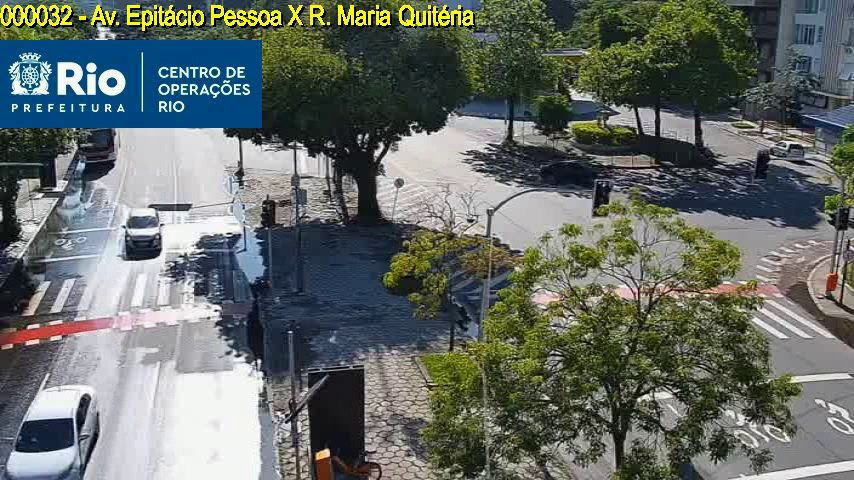
\includegraphics[width=0.8\linewidth]{images/0/CODE32 2023-02-22 08-15-04-6.jpg}}
\caption{Via completamente seca, rotulada como classe 0}
\label{fig:class0_1}
\end{figure}

\begin{figure}[htb]
\centerline{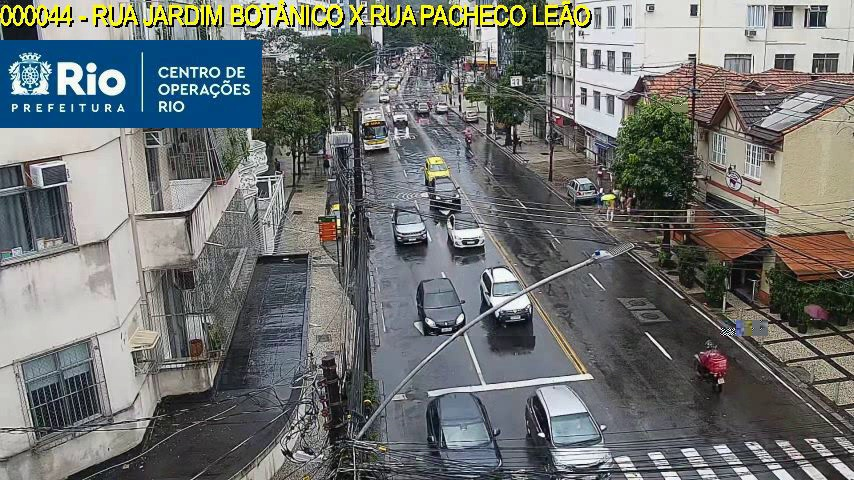
\includegraphics[width=0.8\linewidth]{images/0/CODE44 2023-08-20 13-30-31-6.jpg}}
\caption{Rua molhada, ainda rotulada como classe 0}
\label{fig:class0_2}
\end{figure}

Por outro lado, a Fig. \ref{fig:class1_1} e a Fig. \ref{fig:class1_2} mostram capturas de vias classificadas como \textbf{alagadas}, ou classe 1. 
Em ambas as imagens, é possível ver água cobrindo bastante a rua, dificultando ou impossibilitando a passagem de veículos. 
A Fig. \ref{fig:class1_1} é uma cena capturada pela câmera localizada na zona sul do Rio de Janeiro, no entorno da Lagoa Rodrigo de Freitas. 
A Av. Borges de Medeiros em seu cruzamneto com a Rua Saturnino de Brito, no lado desta lagoa próximo ao bairro Jardim Botânico
A Fig. \ref{fig:class1_1} é o exemplo de uma rua (na zona norte da cidade) parcialmente alagada, dificultante o transito dos veículos onde as calçadas ainda podem ser identificadas. A Fig. \ref{fig:class1_2} é o exemplo de uma rua (da zona sul), sem distinção de calçada ou rua, completamente alagada. Essas situações constituem a classe \textit{alagamento}. 

\begin{figure}[htb]
\centerline{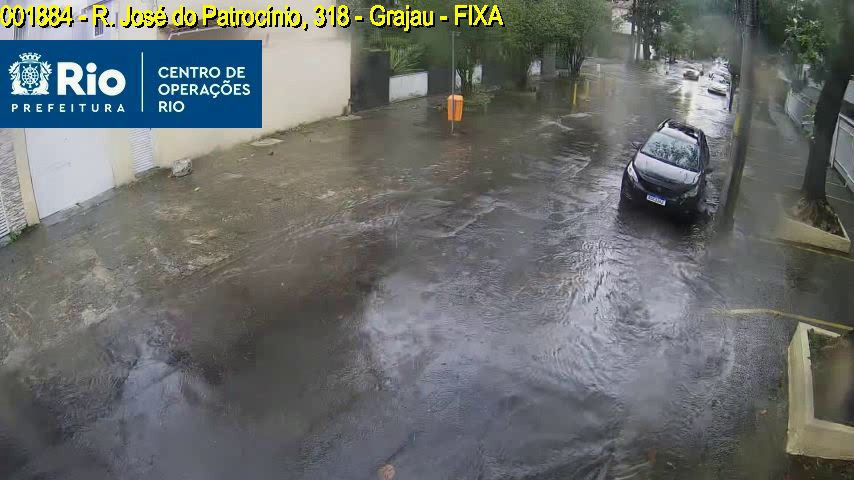
\includegraphics[width=0.8\linewidth]{images/1/CODE1884 2023-08-20 12-56-29-9.jpg}}
\caption{Rua parcialmente alagada (classe 1).}
\label{fig:class1_1}
\end{figure}

\begin{figure}[htb]
\centerline{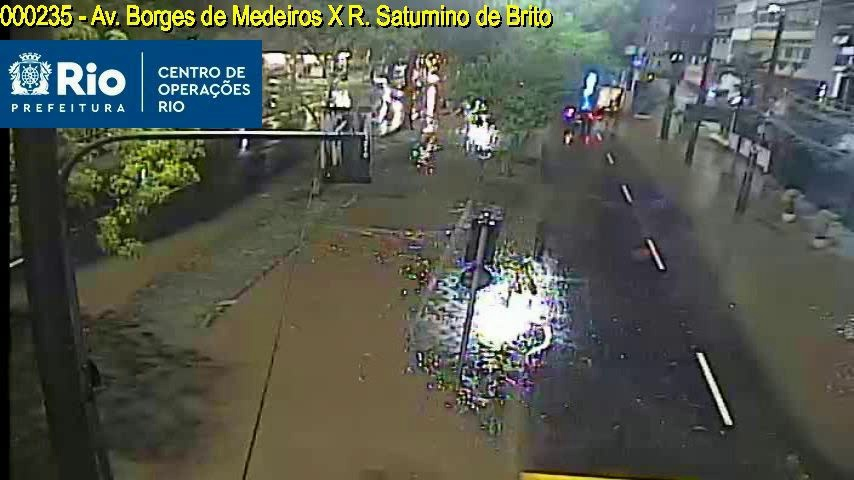
\includegraphics[width=0.8\linewidth]{images/1/CODE235 2023-02-07 20-11-08-9.jpg}}
\caption{Avenida totalmente alagada (classe 1).}
\label{fig:class1_2}
\end{figure}

As Figuras \ref{fig:class0count} e \ref{fig:class1count} mostram a quantidade de imagens (eixo vertical) de cada câmera (eixo horizontal) para a classe 0 e classe 1, respectivamente. 
Essas imagens consistem no conjunto de dados original capturado de 472 câmeras do sistema do \acrshort{cor}, sem balanceamento das classes. 
As imagens de cada classe correspondem as cores, ou seja se identificam em \textbf{alagadas} ou \textbf{não alagadas} de acordo com as cores (azul ou vermelho) de parte das linhas das câmeras mostradas no eixo horizontal do histograma de distribuição. 
Pode-se observar que algumas câmeras possuem muito mais imagens da classe 1 que a outras, provavelmente por ter ocorrido mais chuvas nas regiões onde estas estão localizadas. 
%Ou seja, estarem em regiões (geográficas) onde há maior distribuição de chuvas na cidade do Rio de Janeiro. 
Assim, a criação de um conjunto de dados sem uma análise prévia da representatividade de cada câmera no conjunto possivelmente criaria um viés em qualquer modelo treinado neste conjunto.

% \begin{figure}[htb]
% \centerline{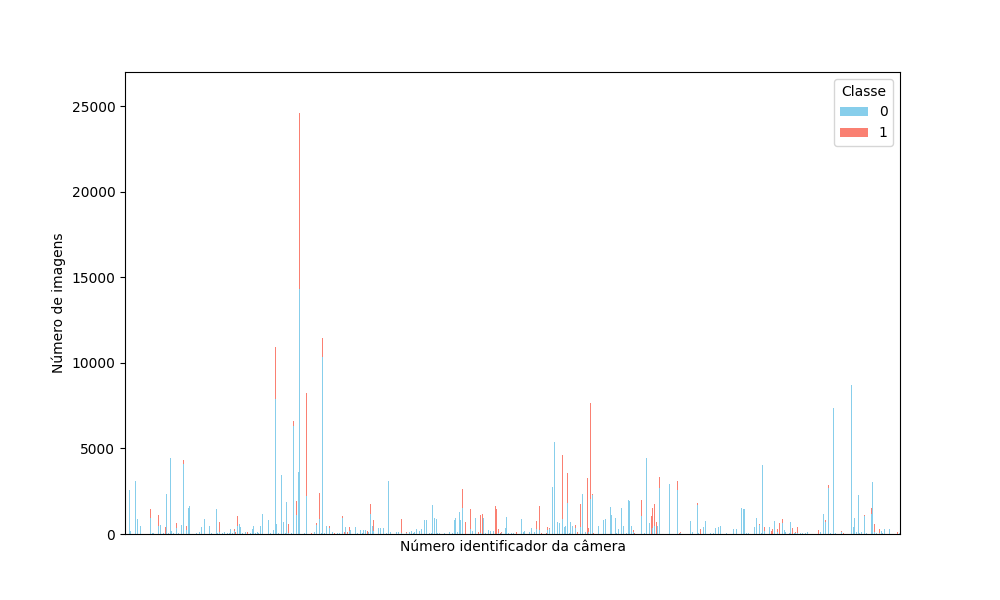
\includegraphics[width=1\linewidth]{images/totalcount_code.png}}
% \caption{Histograma de cada classe por câmera disponível.}
% \label{fig:totalcount}
% \end{figure}

\begin{figure}[htb]
    \centerline{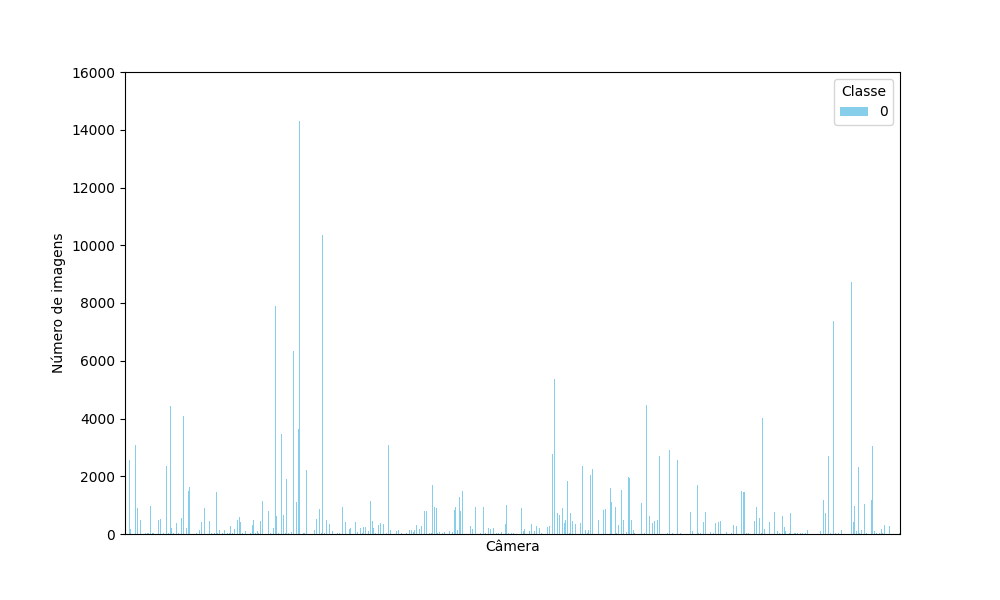
\includegraphics[width=1\linewidth]{images/metodologia/class_0_count_code.png}}
    \caption{Quantidade de imagens de normalidade por câmera disponível.}
    \label{fig:class0count}
\end{figure}

\begin{figure}[htb]
    \centerline{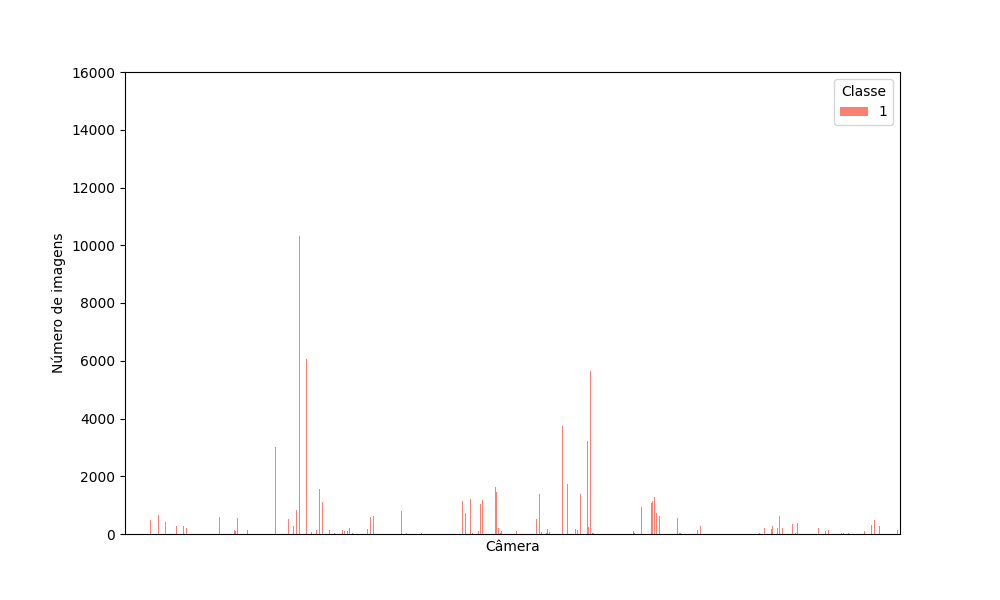
\includegraphics[width=1\linewidth]{images/metodologia/class_1_count_code.png}}
    \caption{Quantidade de imagens de alagamento por câmera disponível.}
    \label{fig:class1count}
\end{figure}

% Diminuindo o limite do eixo vertical, se torna mais claro a quantidade de imagens das demais câmeras, como pode ser visto na Figura \ref{fig:totalcountzoom}. 
% A figura indica a quantidade de imagens de cada classe em cada câmera, com eixo vertical limitado.
A Figura \ref{fig:histcodes} mostra uma distribuição de frequência de câmeras por quantidade de imagens, separadas em intervalos de 100 imagens.
O intervalo com maior ocorrência de câmeras indica o desbalanceamento do conjunto de imagens captadas onde 206 câmeras, ou 43,6\%, possuem até 100 imagens ao todo. 

\begin{figure}[htb]
    \centerline{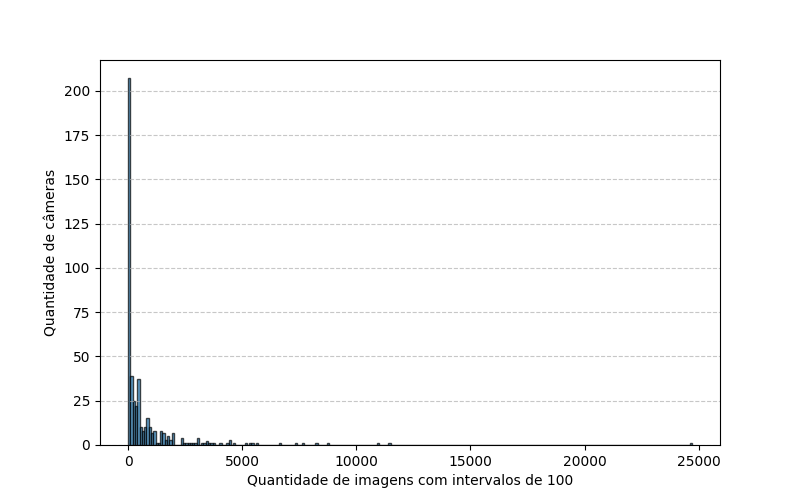
\includegraphics[width=1\linewidth]{images/metodologia/histcodes.png}}
    \caption{Histograma de quantidade de imagens de alagamento por câmera disponível.}
    \label{fig:histcodes}
\end{figure}

Analisando o total de 472 câmeras, 330 delas possuem menos de 500 imagens registradas de ambas as classes, ou 69,9\% das câmeras.
Vale ressaltar que esses dados não levam em conta a proporção de imagens de cada classe no total em cada câmera.

% \begin{figure}[htb]
% \centerline{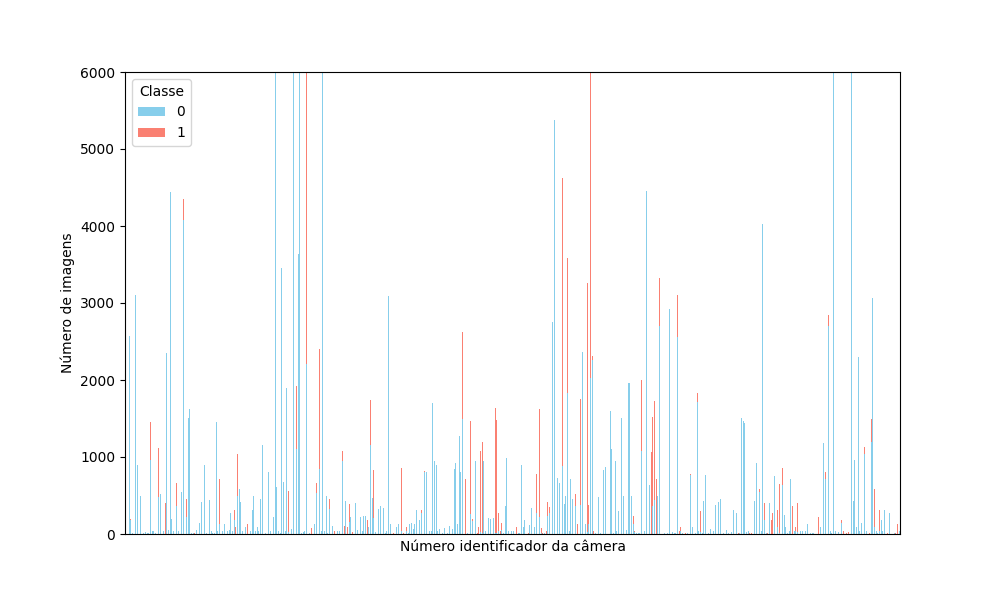
\includegraphics[width=1\linewidth]{images/totalcountzoom_code.png}}
% \caption{Histograma com eixo vertical limitado.}
% \label{fig:totalcountzoom}
% \end{figure}

Diante do exposto, foi necessário considerar qual a quantidade de imagens de cada classe por câmera deve ser considerada para criar um conjunto de dados balanceado e diverso em sua representatividade de câmeras de lugares diferentes. 
Para isso, foi analisada a quantidade de câmeras que possui um determinado número mínimo de imagens para cada classe, permitindo saber quantas imagens e qual seria a variedade de um conjunto de dados balanceado formado com as imagens captadas e classificadas.

A Figura \ref{fig:balancedcodes} mostra a quantidade de câmeras para a condição descrita. 
Inicialmente, foi julgado que 10 imagens de cada classe por câmeras formaria um conjunto de dados com relativamente poucas imagens levando em consideração as outras possíveis quantidades de imagens por câmera, compondo um conjunto de dados de 1800 imagens, visto que há 90 câmeras com pelo menos 10 imagens de cada classe. 
Um conjunto de dados com 50 imagens de cada classe forneceria 60 câmeras, para um total de 6000 imagens, entretanto, o conjunto de dados ficaria muito maior e com menor variedade de câmeras que usar, por exemplo, o valor escolhido de 30 imagens por câmeras, que teria 77 câmeras. 

\begin{figure}[htb]
\centerline{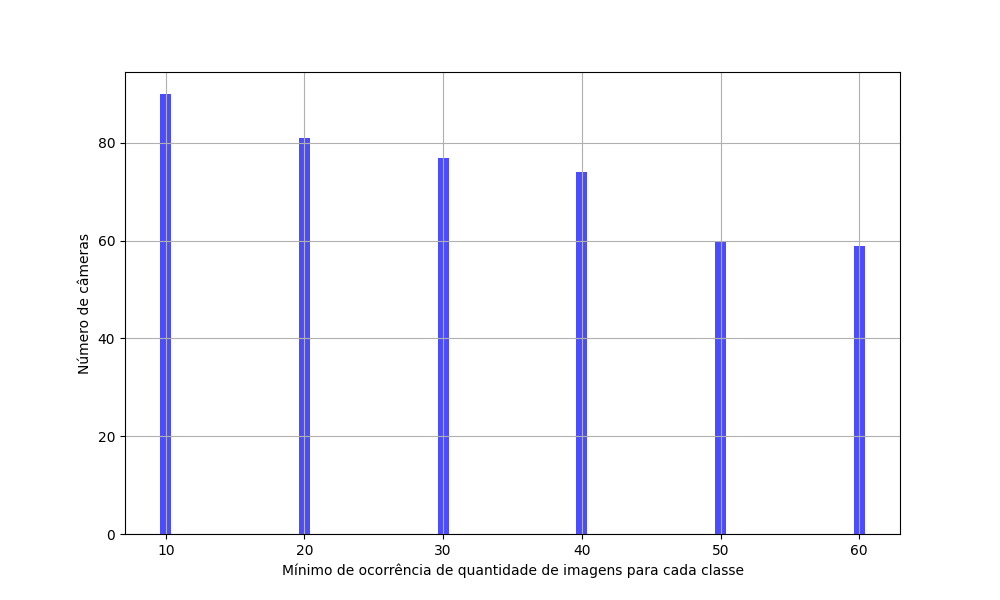
\includegraphics[width=1\linewidth]{images/balancedcodes.png}}
\caption{Quantidade de câmeras com um número mínimo de imagens de cada classe.}
\label{fig:balancedcodes}
\end{figure}

Ao final da avaliação dos modelos de \acrshort{cnn}s, uma reavaliação do número de imagens por câmeras é refeito para tomar uma decisão certa sobre a melhor quantidade de imagens por câmeras, 
e se essa mudança acarretaria melhora nos índices usados para avaliação do modelo, como é apresentado na seção \ref{sec:cameraquantity}.
% -----------------------
\subsection{Pré Processamento}\label{subsec:datapreprocessing}

Diversas etapas de pré-processamento foram aplicadas para melhorar a qualidade das imagens no conjunto de dados.

Primeiramente, uma máscara foi aplicada para remover o logotipo do \acrshort{cor} (ou seja, a região superior esquerda com os brasão da cidade e palavras brancas sobre um fundo azul) das imagens para evitar que o logotipo enviesasse o processo de aprendizado do modelo. Isso foi feito zerando a região da imagem onde o logotipo do COR está localizado, já que sua posição é estática. Como o logotipo está presente em todos os quadros, não foi possível recriar a região apagada com quadros intermediários.

Segundo, como algumas imagens podem apresentar brilho excessivo, os canais de imagem $RGB$ originais foram convertidos para o espaço de cor $YC_rC_b$ para permitir o ajuste no canal \textit{Y}, 
reduzindo o brilho da imagem. Essa transformação no canal \textit{Y} foi feita multiplicando os valores de pixel no canal \textit{Y} por um fator de brilho, 
um número real positivo mas menor que 1, com um valor inicial de 0,5. 

Então, cada informação de pixel $YC_rC_b$ é convertida de volta para  \textit{RGB}, para ser mostrada nas telas do computador colorida como originalmente. 
Entretanto, outros valores de fator de brilho (FB) foram avaliados posteriormente na seção \ref{sec:bestmodel}.
As Figuras \ref{fig:samplebright} e \ref{fig:samplebright_half} mostram a mesma cena de um local onde o FB foi aplicado. 
É possível notar a diferença na intensidade do brilho da cena após a alteração no canal \textit{Y}.

\begin{figure}[htb]
    \centerline{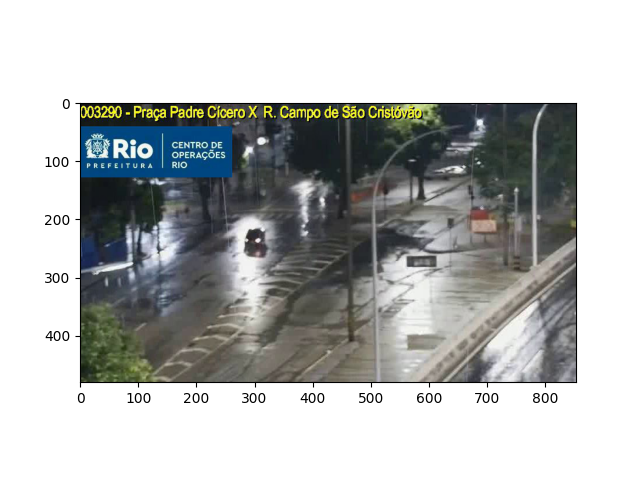
\includegraphics[width=1\linewidth]{images/metodologia/samplebright.png}}
    \caption{Exemplo de região sem alteração no canal \textit{Y}.}
    \label{fig:samplebright}
\end{figure}
\begin{figure}[htb]
    \centerline{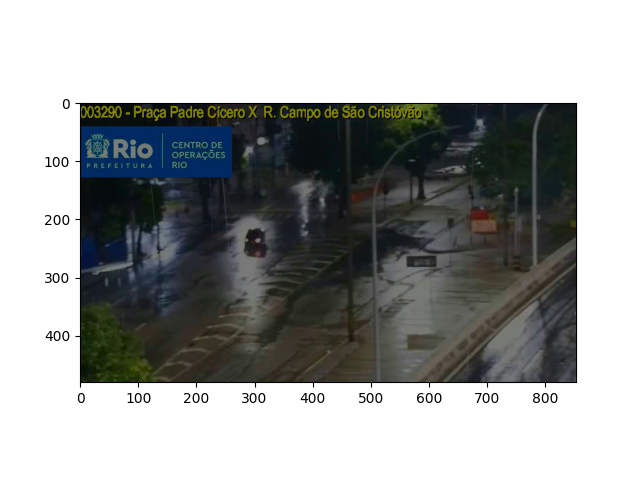
\includegraphics[width=1\linewidth]{images/metodologia/samplebright_half.png}}
    \caption{Exemplo de mesma região com 50\% do valor original de \textit{Y}.}
    \label{fig:samplebright_half}
\end{figure}

%\textbf{Sim precisa fazer isso. Veja que  esse processamento se chama de unsharp masking na literatura , por exemplo LIM, Gonzales, Sonka, etc . E deveria estar na seção de metodologia}

%\textbf{André. isso que fala no inicio do próximo paragrafo deveria ficar em um dos capítulos iniciais, veja que perguntei isto, em relação ao tipo de câmera. Em dissertações você deve é pode ser prolixo, isso não é artigo com máximo de paginas fixas!  Aqui tem que se proteger do membro da banca ler correndo e nem notar algo importante como isso que aqui descreve} 

Para introduzir mais variedade às imagens no treinamento, em seguida foi aplicada uma inversão horizontal aleatória foi aplicada com uma probabilidade de 50\% nos dados de entrada.
Em outras palavras, cada imagem da divisão de treinamento tem 50\% de chance de ser invertida horizontalmente ou não.

Além disso, transformações padrões de redimensionamento, corte e normalização de intensidades são usadas para preparar as imagens para cada modelo $CNN$. 
É aplicado aos dados inicialmente um processo de redimensionamento para transformar cada quadro ajustado ao tamanho esperado de cada modelo,
onde as imagens com dimensão 854 x 480 pixels são redimensionadas para 256 x 256 pixels. 
Então eles são submetidos a um corte de dimensão 224 x 224 pixels de mesmo centro da imagem.
Com exceção do \textit{Inception}, que redimensiona para 342 x 342 pixels e realiza um corte central de 299 x 299 pixels.
Os valores do conteúdo de cada pixel são redimensionados para estarem no intervalo [0,1]. 

%\textit{Andre(não entendi nada do que foi feito pelo falado no próximo paragrafo) RE ESCREVE}

Finalmente, todo o conjunto de dados foi normalizado pela média e desvio padrão específicos de cada modelo:
Todos os modelos avaliados têm a mesma matriz média de (0,485 ; 0,456 ; 0,406) e matriz de desvio padrão de (0,229 ; 0,224 ; 0,225) para cada canal $RGB$, usados para normalizar a imagem. 
%Da mesma forma, eles também compartilham o mesmo tamanho de imagem de 256$\times$256. Com exceção do InceptionV3, que tem tamanho de imagem de 342$\times$342.
% ----------------------------------------------------------
\section{Modelos de classificação}\label{sec:methodology_models}

Com base na nos trabalhos da literatura sobre alagamento urbano anteriormente apresentados, os modelos MobileNetV2 \cite{mobilenetv2}, VGG19 \cite{vgg}, InceptionV3 \cite{inception} e DenseNet \cite{densenet} foram avaliados.
Além disso, a arquitetura de \acrfull{vit}\cite{vit} foi incluída. Essa adição foi feita porque vários modelos de classificação de imagens de alto desempenho são baseados em arquiteturas $Visual$ $Transformers$, como $ViT-Huge$ usado no conjunto de dados CIFAR-10 \cite{dosovitskiy2021image} e $ViT-Large$ no conjunto de dados STL-10 \cite{gesmundo2022continual, kabir2023reduction}.

Todos os modelos foram treinados em 50 épocas, onde o \textit{Early Stopping} foi empregado com uma restrição de 10 épocas e decaimento da taxa de aprendizagem de 0,1. Três diferentes taxas de aprendizagem foram aplicadas em todos os modelos, visto que as diferentes complexidades dos modelos podem resultar em diferentes taxas de aprendizagem ótimas. O \acrfull{sgd} foi usado como otimizador inicialmente, entretanto, outros otimizadores foram testados após a avaliações dos modelos, como pode ser visto na seção \ref{sec:optimizer}.

A transferência de aprendizado foi aplicada a todos os modelos, inicializando-os com os pesos padrões do IMAGENET. Isso foi feito para utilizar os pesos aprendidos anteriormente para auxiliar no aprendizado dos pesos das novas classes \cite{kolesnikov2020big}. Posteriormente, a última camada totalmente conectada foi modificada para ter apenas duas saídas, se adequando ao problema de classificação binária.
% ----------------------------------------------------------
\section{Avaliação dos modelos}

Para avaliar o desempenho dos cinco modelos com diferentes taxas de aprendizagem, inicialmente foi utilizado a acurácia para distinguir o melhor modelo. 
Após a identificação do melhor modelo, a precisão e revocação também foi utilizada para melhor entender seu desempenho. 

Como o conjunto de dados está completamente balanceado, conforme mencionado na Seção \ref{sec:dataset}, com ambas as classes igualmente representativas, esses avaliadores fornecem um cenário adequado para compreensão dos resultados. Adicionalmente, todas as câmeras possuem o mesmo número de imagens, garantindo assim uma representação equilibrada entre as fontes de dados e suas distribuições pela cidade.

Para calcular a acurácia, precisão e revocação, inicialmente foram obtidos os seguintes valores: 
Verdadeiros Positivos (TP), que correspondem ao número de rótulos positivos classificados corretamente pelo modelo; 
Verdadeiros Negativos (TN), que representam os rótulos negativos classificados corretamente; 
Falsos Positivos (FP), que são os rótulos positivos classificados incorretamente; 
e Falsos Negativos (FN), que indicam o número de rótulos negativos classificados de forma incorreta.

O primeiro índice de avaliação selecionada para análise foi a acurácia, 
pois ela fornece uma visão geral da capacidade do modelo em classificar corretamente os exemplos em um conjunto de dados balanceado. 
%Como o objetivo inicial deste estudo é representar com precisão a situação de inundação nas ruas, a precisão e a revocação também foram escolhidas como métricas apropriadas para complementar a análise.

A acurácia pode ser calculada pela seguinte fórmula:
\begin{equation}
    \label{eqn:accuracy}
    Acuracia = \frac{TP+TN}{TP+TN+FP+FN}
\end{equation}

O índice de avaliação de precisão indica a porcentagem de imagens classificadas como positivas que realmente pertencem à classe positiva \cite{FAWCETT2006861}. 
É especialmente relevante para aumentar a confiabilidade do modelo na identificação correta da situação de inundação.

%A precisão é um indicativo da proporção de classificações positivas corretas em relação ao total de predições positivas, e é uma medida importante em contextos onde a minimização de falsos positivos é desejável.%
A Equação \ref{eqn:precision} formaliza o cálculo da precisão:
\begin{equation}
    \label{eqn:precision}
    Precisao = \frac{TP}{TP+FP}
\end{equation}

Além disso, a revocação pode ser empregada como um avaliador final para calcular a taxa de imagens positivas classificadas corretamente \cite{MurphyProbabilistic}. 
Ela é útil para garantir que o menor número possível de situações de inundação seja classificado incorretamente. A revocação mede a capacidade do modelo de identificar corretamente todas as instâncias relevantes.
A equação a seguir define o cálculo da revocação:
\begin{equation}
    \label{eqn:recall}
    Revocacao = \frac{TP}{TP+FN}
\end{equation}

O próximo capitulo apresenta os resultados obtidos. 

\pagestyle{ruledheader}
\chapter{Experimentos e Resultados}\label{cap:resultados}
Esta seção apresenta os resultados das cinco arquiteturas analisadas.
Em seguida, a arquitetura com melhor desempenho é analisada mais detalhadamente sob diferentes aspectos.
Toda a pesquisa foi realizada em uma máquina com placa gráfica NVIDIA GeForce RTX 3060 Ti, processador Intel Core i7-11700K de 3,60 GHz e 16 GB de memória RAM.
% ----------------------------------------------------------
\section{Resultados dos Modelos}\label{sec:modelsresults}

A Tabela \ref{tab:metrics} exibe a acurácia de cada modelo com diferentes taxas de aprendizagem, utilizando o \acrshort{sgd} como otimizador.
A taxa de aprendizagem de 1x10$^{-5}$ apresentou as melhores acurácias no geral, porém não gerou o melhor modelo.
Nenhum modelo obteve boa acurácia com essa taxa de aprendizagem, indicando que um valor muito baixo limitou a capacidade dos modelos de convergir para uma solução satisfatória.

O \textit{MobileNetV2} obteve os piores resultados nas outras duas taxas de aprendizagem avaliadas.
Já o \acrshort{vit} apresentou o melhor desempenho, com acurácia superior tanto para a taxa de aprendizagem de 1x10$^{-3}$ quanto para a de 1x10$^{-4}$.

\begin{table}[tb]
\caption{\label{tab:metrics} Acurácia dos cinco modelos com diferentes taxas de aprendizagem.}
\begin{center}
\begin{tabular}{c|ccc}
\toprule
\multirow{2}{*}{Modelos} & \multicolumn{3}{c}{Taxa de aprendizagem}   \\
                         & 1x10-03     & 1x10-04     & 1x10-05     \\
\midrule
VGG19                    & 0,808 & 0,732 & 0,524 \\
\midrule
InceptionV3              & 0,795     & 0,731     & 0,529        \\
\midrule
DenseNet                 & 0,802     & 0,658     & 0,592     \\
\midrule
MobileNetV2              & 0,781  & 0,608 & 0,534 \\
\midrule
ViT                      & 0,816     & \textbf{0,826}     & 0,511     \\
\bottomrule
\end{tabular}
\end{center}

\end{table}

O desempenho inferior do \textit{MobileNetV2} pode ser explicado por sua arquitetura, projetada para uso em dispositivos com menor poder computacional \cite{mobilenetv2}, possuindo, portanto, um número significativamente menor de parâmetros treináveis em comparação com as demais arquiteturas avaliadas.

Um comportamento comum a todos os modelos, exceto o \acrshort{vit}, foi a redução da acurácia conforme a diminuição da taxa de aprendizagem.
Isso sugere que taxas de aprendizagem muito baixas podem ser inadequadas para ajustar a grande quantidade de parâmetros presentes em redes profundas.

Apesar de tanto o \acrshort{vgg} quanto o \textit{DenseNet} terem alcançado acurácias próximas a 80\%, o \acrshort{vit} apresentou resultados ligeiramente superiores.
Outro aspecto relevante a ser considerado é que, enquanto o \textit{InceptionV3} levou 47 minutos para completar seu treinamento, o \acrshort{vit} realizou o mesmo em apenas 22 minutos no mesmo conjunto de dados.
Portanto, o \acrshort{vit} utilizando taxa de aprendizado de 1x10$^{-4}$ foi selecionado como o modelo a ser utilizado para as etapas subsequentes deste trabalho.
% ----------------------------------------------------------

\section{Avaliação do melhor modelo}\label{sec:bestmodel}

Após a escolha da arquitetura de melhor desempenho e da taxa de aprendizado adequada, outras análises devem ser feitas para saber se é possível melhorar seus resultados e o quão adequado foi seu treinamento.

% -----------------------

\subsection{Validação cruzada K-Fold}

A primeira análise realizada exclusivamente com o \acrshort{vit} foi a aplicação de validação cruzada do tipo K-Fold, utilizando o mesmo conjunto de dados.
A Tabela \ref{tab:kfold} apresenta as métricas de acurácia, precisão e revocação obtidas nos cinco subconjuntos, ou \textit{folds}, empregados na validação.

A acurácia média de 0,801 obtida na validação cruzada foi inferior à acurácia de 0,826 observada na validação simples.
Esse resultado sugere que o conjunto de treino inicialmente utilizado pode ter incluído imagens mais facilmente classificáveis, o que beneficiou o desempenho na validação simples.

Ao analisar cada subconjunto individualmente, observa-se que os folds 2 e 5 apresentaram acurácias significativamente menores em relação aos demais.
Tal comportamento indica que as características das câmeras incluídas nesses subconjuntos de validação não foram adequadamente aprendidas pelo modelo, que foi treinado com imagens provenientes das outras câmeras.
Além disso, a baixa revocação observada no subconjunto 5 pode indicar que o modelo adotou uma estratégia conservadora, prevendo a classe de normalidade apenas em situações de classificação com maior confiança, ao custo do aumento de falsos negativos.

Embora o modelo tenha mantido uma acurácia média aceitável, o desempenho inferior nos subconjuntos 2 e 5 evidencia uma sensibilidade dos resultados à composição das câmeras no conjunto de treino, ressaltando a importância de uma seleção equilibrada das câmeras para garantir generalização adequada do modelo.
% \usepackage{graphicx}
\begin{table}[tb]
\caption{\label{tab:kfold} Métricas do ViT com validação cruzada K-Fold com K=5.}
% \resizebox{\columnwidth}{!}{%
\begin{center}
\begin{tabular}{c|ccc}
\toprule
Subconjunto  & Acurácia & Precisão & Revocação \\
\midrule
1     & 0,833    & 0,838    & 0,827     \\
\midrule
2     & 0,777    & 0,773    & 0,785     \\
\midrule
3     & 0,794    & 0,780    & 0,820     \\
\midrule
4     & 0,819    & 0,801    & 0,849     \\
\midrule
5     & 0,771    & 0,816    & 0,700     \\
\midrule
Média & 0,794    & 0,801    & 0,820     \\
\bottomrule
\end{tabular}%
\end{center}
%}
\end{table}

% -----------------------

\subsection{Métricas no conjunto de teste}

Após a validação cruzada, o modelo também foi avaliado no conjunto de teste, o qual apresenta balanceamento entre as classes, porém não possui balanceamento na quantidade de imagens provenientes de cada câmera que compõe esse conjunto.

A Tabela \ref{tab:test} exibe os resultados obtidos pelo modelo no conjunto de teste, juntamente com seus resultados na validação cruzada.
Observa-se uma leve queda na acurácia, contudo o modelo mantém uma capacidade razoável de classificação.
O aumento na precisão indica que o modelo cometeu menos falsos positivos no conjunto de teste, evidenciando uma classificação mais conservadora da classe positiva.

Entretanto, houve uma queda significativa na revocação no conjunto de teste.
Dessa forma, apesar da postura conservadora, o modelo falhou em classificar corretamente uma quantidade expressiva de verdadeiros positivos.

\begin{table}[tb]
\caption{\label{tab:test} Métricas do ViT no conjunto de teste.}
\begin{center}
\begin{tabular}{c|ccc}
\toprule
Conjunto          & Acurácia & Precisão & Revocação \\
\midrule
Validação Cruzada & 0,794    & 0,801    & 0,820     \\
\midrule
Teste             & 0,780    & 0,814    & 0,719     \\
\bottomrule
\end{tabular}%
\end{center}
\end{table}
% -----------------------

\subsection{Diminuição da intensidade luminosa}
Após a escolha da arquitetura de melhor desempenho, diferentes valores para o fator denominado nesta dissertação como fator de claridade (\textit{FC}), conforme mencionado na Seção \ref{subsec:datapreprocessing}, foram avaliados utilizando o \acrshort{vit}, com o objetivo de analisar se o modelo poderia ser aprimorado ao levar em consideração a claridade excessiva presente em algumas imagens.

A Tabela \ref{tab:brightnessfactor} apresenta o desempenho do \acrshort{vit} com quatro valores distintos para o \textit{FC}, sendo que o valor 1 para o \textit{FC} indica que a intensidade luminosa da imagem não foi alterada, ou seja, a quantidade de regiões com pixels na cor branca permanece inalterada em relação à imagem original.
A redução do \textit{FC} promoveu uma melhora gradual no desempenho do modelo, entretanto, um \textit{FC} muito baixo impactou negativamente o resultado, como evidenciado pelos resultados obtidos com \textit{FC} igual a 0,25.
A diminuição do \textit{FC} para 0,75 gerou uma melhora marginal nos resultados, contudo a escolha inicial de 0,5 mostrou-se a mais adequada dentre os valores testados.

\begin{table}[tb]
\caption{\label{tab:brightnessfactor} Redução de áreas de brancos e desempenho do \acrshort{vit}}
\begin{center}
\begin{tabular}{c|ccc}
\toprule
 Fatores de claridade & Acurácia &  Precisão  & Revocação \\
\midrule
     0,25 & 0,703 & 0,758 & 0,604 \\
     0,5 & \textbf{0,826} & \textbf{0,863} & \textbf{0,778} \\
     0,75 & 0,769 & 0,802 & 0,738 \\
     1 & 0,756 & 0,782 & 0,708 \\
\bottomrule
\end{tabular}
\end{center}
\end{table}

\subsection{Curvas de acurácia e perda do melhor modelo}
A Figura \ref{fig:acc} e a Figura \ref{fig:loss} apresentam o desempenho do \acrshort{vit} durante as fases de treinamento (linha azul) e validação (linha vermelha).

No treinamento, a acurácia (Figura \ref{fig:acc}) converge para aproximadamente 0,87, enquanto na validação mantém-se em torno de 0,83.
Entretanto, ao observar apenas a acurácia no conjunto de validação, nota-se que ela iniciou com valores relativamente altos antes de convergir.
A pequena discrepância entre as acurácias de treinamento e validação indica que não houve $overfitting$ dos dados, demonstrando que o modelo foi capaz de generalizar adequadamente.

Ao analisar a perda (\textit{loss}) durante o treinamento (Figura \ref{fig:loss}), observa-se que, apesar da alta acurácia no conjunto de treino, a perda permaneceu relativamente elevada inicialmente, estabilizando-se em torno de 0,37 (linha azul), enquanto a perda no conjunto de validação estabilizou-se em aproximadamente 0,43 (linha vermelha).

\begin{figure}[tb]
\centerline{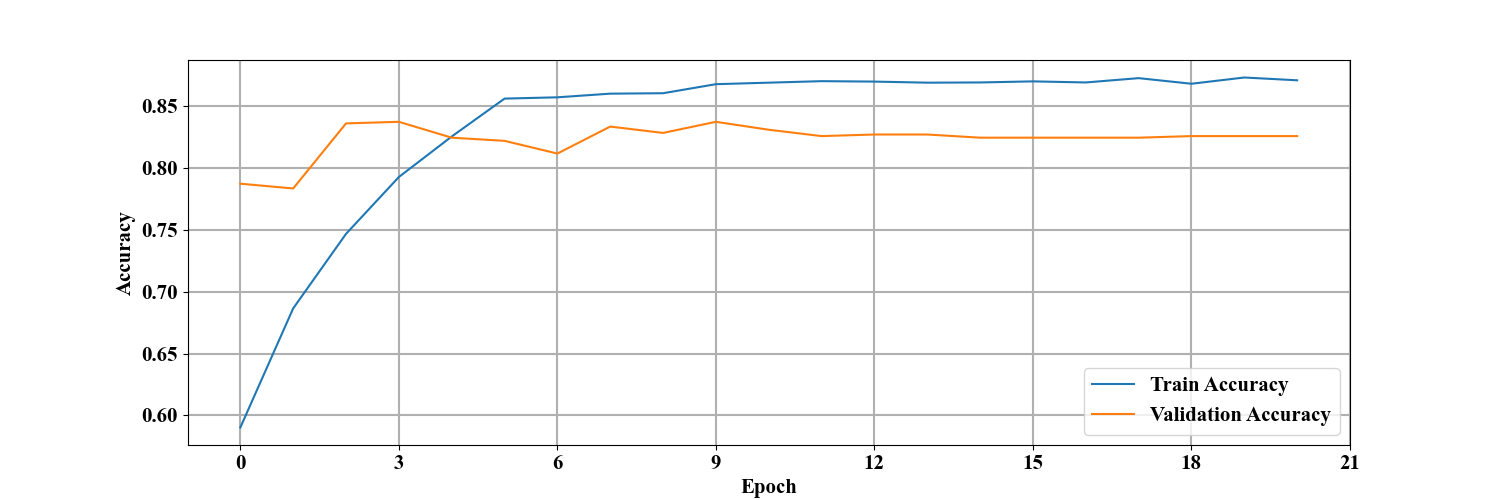
\includegraphics[width=1\linewidth]{images/resultados/sgd_accuracy.png}}
\caption{Acurácia do \acrshort{vit} durante treino e validação.}
\label{fig:acc}
\end{figure}

\begin{figure}[tb]
\centerline{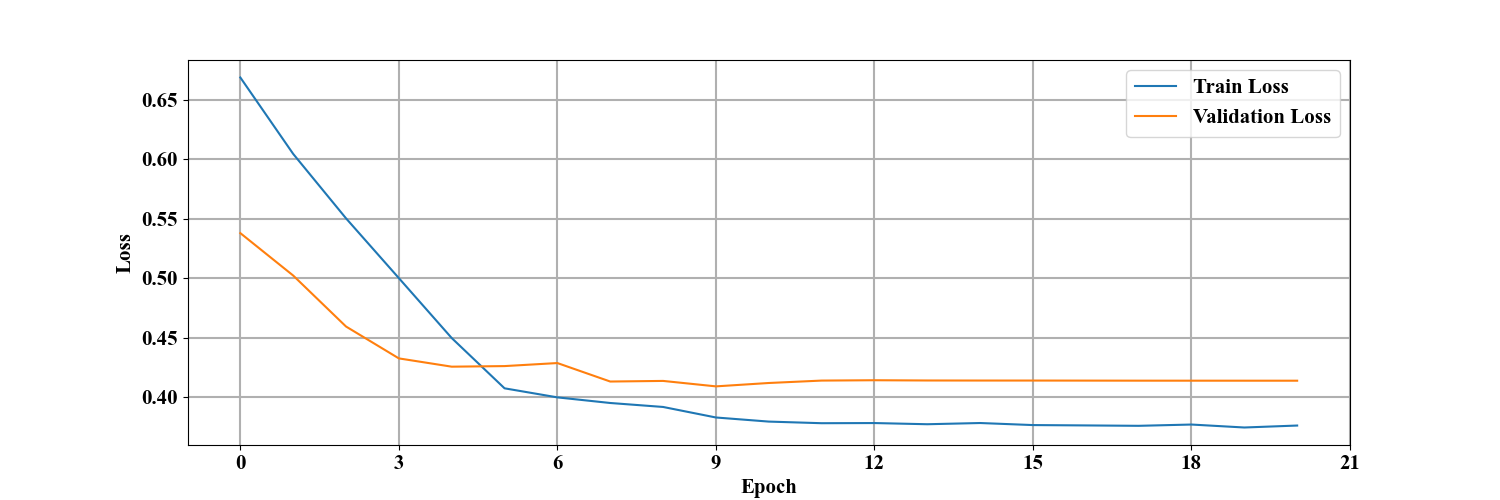
\includegraphics[width=1\linewidth]{images/resultados/sgd_loss.png}}
\caption{Perda do \acrshort{vit} durante treino e validação.}
\label{fig:loss}
\end{figure}

A pequena diferença na acurácia entre os conjuntos de treinamento e validação (Fig. \ref{fig:acc}) pode ser justificada pela introdução de características no conjunto de validação que não estão presentes no conjunto de treinamento.

% ----------------------------------------------------------
\subsection{Melhor modelo com diferentes quantidades de câmeras}\label{sec:cameraquantity}

Com o objetivo de verificar se o aumento da quantidade de câmeras no conjunto de treino levaria a melhorias significativas em sua performance, a arquitetura \acrshort{vit} foi treinada com conjuntos de treino menores.
Esses conjuntos possuem menor quantidade de câmeras, mas mantêm o mesmo número de imagens por classe para cada câmera.

Para compor esses conjuntos comparativos ao utilizado originalmente, dentre as 60 câmeras que compõem o conjunto original, foram escolhidas aleatoriamente 30 câmeras para formar o segundo conjunto.
Dessas 30 câmeras, foram selecionadas aleatoriamente 15 para compor o terceiro conjunto.
Portanto, os três conjuntos de treino possuem as mesmas 15 câmeras, e o conjunto com 60 câmeras inclui todo o conjunto das 30 câmeras, acrescido de outras 30 câmeras adicionais.

Dessa forma, o efeito de adicionar novas câmeras ao conjunto de treino pode ser mais facilmente compreendido.
A Tabela \ref{tab:trainingimages} apresenta a relação entre o tamanho do conjunto de treino, sua acurácia e o tempo de treinamento.
O modelo foi testado utilizando o mesmo conjunto de teste pertencente ao conjunto de dados original.

\begin{table}[!ht]
\begin{center}
\caption{Acurácia $\times$ tempo de treino $\times$ número de imagens usadas}
\label{tab:trainingimages}
\begin{tabular}{c|cc}
%\hline
\toprule
\textbf{\textbf{Nº de Câmeras}} & \textbf{Acurácia} & \textbf{Tempo (minutos)}\\
%\hline\hline
\midrule
15 &  0,728 & 17\\
30 & 0,804 & 18 \\
60 & 0,826 & 21 \\
%\hline
\bottomrule
\end{tabular}
\end{center}
\end{table}

Como esperado, aumentar a diversidade de câmeras no conjunto de treino e, consequentemente, a quantidade total de imagens de treino, resultou em incremento na acurácia do modelo.
Entretanto, o número de câmeras atualmente utilizado mostra-se adequado, pois a inclusão de mais câmeras não trouxe melhorias significativas no desempenho.
Observou-se que dobrar a quantidade de imagens de treino, passando de 1800 para 3600 — ou seja, de 30 para 60 câmeras no conjunto de treino — representou uma melhoria marginal de apenas 0,022 na acurácia.

% ----------------------------------------------------------

\section{Comparação entre diferentes otimizadores}\label{sec:optimizer}
Apesar de, inicialmente, todos os modelos terem sido treinados utilizando o \acrshort{sgd} como otimizador, a escolha de diferentes otimizadores e taxas de aprendizagem pode influenciar significativamente a performance das \acrshort{cnn}.

Com base nos resultados apresentados por Dogo \textit{et al.} \cite{Dogo2022optimizers}, que compararam diversos otimizadores em redes neurais e conjuntos de dados de diferentes tamanhos e complexidades, esta dissertação realizou uma comparação dos resultados do \acrshort{vit} utilizando o \acrshort{sgd}, o \acrlong{adam} \cite{adam} e o \acrlong{nadam} \cite{nadam}.
Todos os otimizadores foram configurados conforme descrito na Seção \ref{sec:methodology_models}, sendo testados com diferentes taxas de aprendizagem iniciais.

\begin{table}[tb]
%\resizebox{\columnwidth}{!}{%
\caption{\label{tab:optimizer_acc} Acurácia do \acrshort{vit} com diferentes otimizadores.}
\begin{center}
\begin{tabular}{c| c c c }
\toprule
\multirow{2}{*}{\begin{tabular}[c]{@{}c@{}}Taxa de \\ Aprendizado\end{tabular}} & \multicolumn{3}{c}{Acurácia}   \\
                                                                                & SGD      & Adam     & NAdam    \\
\midrule
1x10-06                                                                           & 0,504   & 0,833 & 0,819 \\
1x10-05                                                                           & 0,512 & 0,841 & \textbf{0,862} \\
1x10-04                                                                           & 0,826 & 0,636 & 0,650    \\
\bottomrule
\end{tabular}
\end{center}%
%}
\end{table}

\begin{figure}[tb]
\centerline{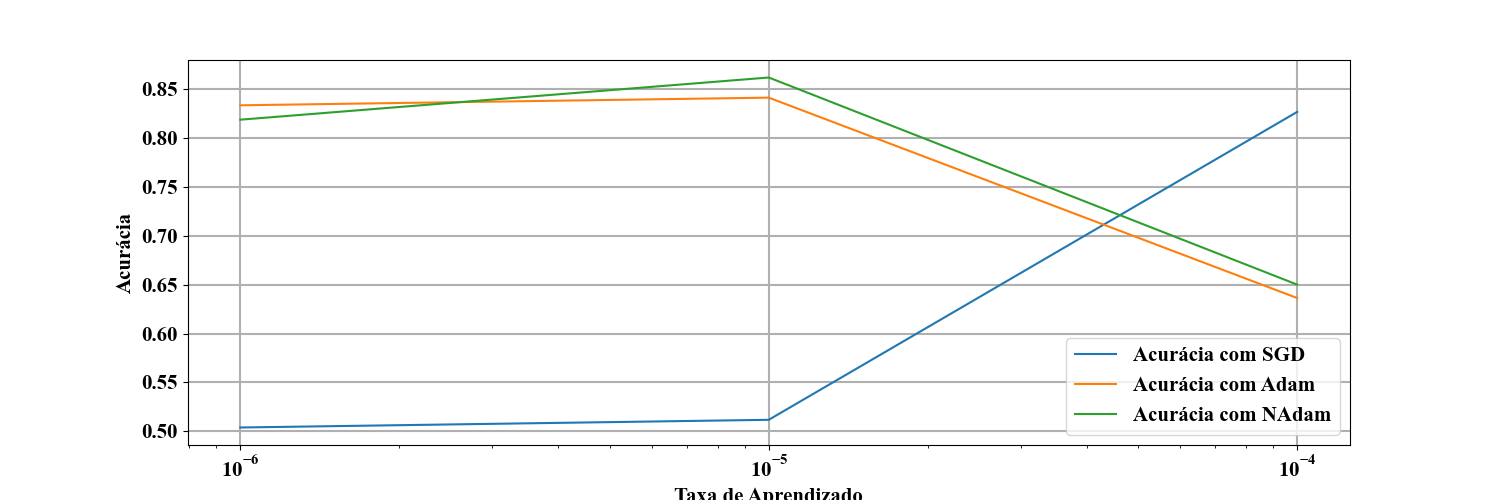
\includegraphics[width=1\linewidth]{images/resultados/optimizer_acc.png}}
\caption{Acurácia do \acrshort{vit} com diferentes otimizadores.}
\label{fig:optmizer_acc}
\end{figure}

Os resultados apresentados na Tabela \ref{tab:optimizer_acc} indicam que tanto o \acrshort{adam} quanto o \acrshort{nadam} apresentaram acurácias superiores ao \acrshort{sgd}.
O \acrshort{nadam} obteve a melhor acurácia, alcançando 0,86 com uma taxa de aprendizado de 1x10$^{-5}$.

Ao analisar o desempenho do \acrshort{sgd}, observa-se que taxas de aprendizado menores resultaram em piores resultados, possivelmente indicando que o passo de atualização foi muito pequeno para escapar de mínimos locais, especialmente em arquiteturas mais complexas, como o \acrshort{vit}.

Nenhum dos otimizadores conseguiu obter um bom desempenho com a menor taxa de aprendizado, o que pode ser explicado pelo fato de que o modelo não realizou atualizações significativas nos pesos durante o treinamento.
As variantes do \acrshort{adam} apresentaram melhor performance com taxas de aprendizado moderadas, com o \acrshort{nadam} se destacando.
A utilização da aceleração de Nesterov para atualizações mais rápidas no \acrshort{nadam} pode ser a principal responsável por seu desempenho superior.

As Figuras \ref{fig:nadam_acc} e \ref{fig:nadam_loss} ilustram a acurácia e a perda do \acrshort{vit} durante o treinamento com o \acrshort{nadam}, utilizando a taxa de aprendizado de 1x10$^{-5}$, momento em que foi obtida a maior acurácia de validação.
Considerando que o modelo estabilizou sua acurácia de treinamento em 1 , enquanto a acurácia de validação se manteve em torno de 0,862, observa-se que o modelo não conseguiu generalizar adequadamente, indicando a ocorrência de \textit{overfitting}.
Esse fenômeno é corroborado pela curva de perda, na qual a perda de validação aumentou, em contraste com a perda de treinamento, que diminuiu para valores próximos a zero.

\begin{figure}[tb]
\centerline{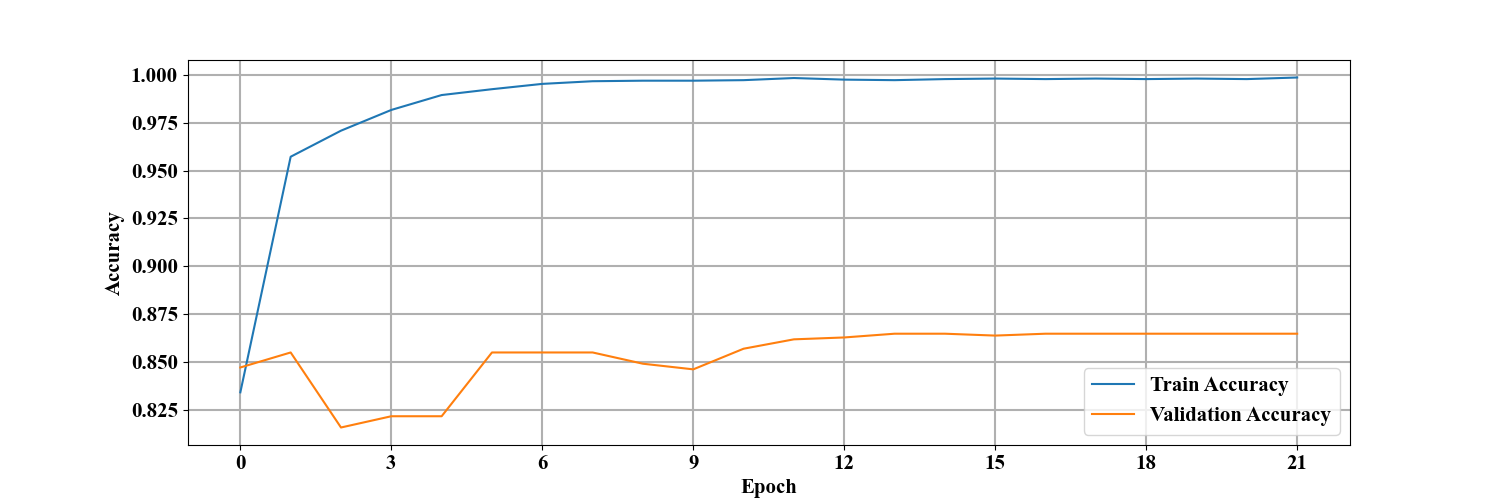
\includegraphics[width=1\linewidth]{images/resultados/nadam_accuracy.png}}
\caption{Acurácia do \acrshort{vit} com NAdam.}
\label{fig:nadam_acc}
\end{figure}

\begin{figure}[tb]
\centerline{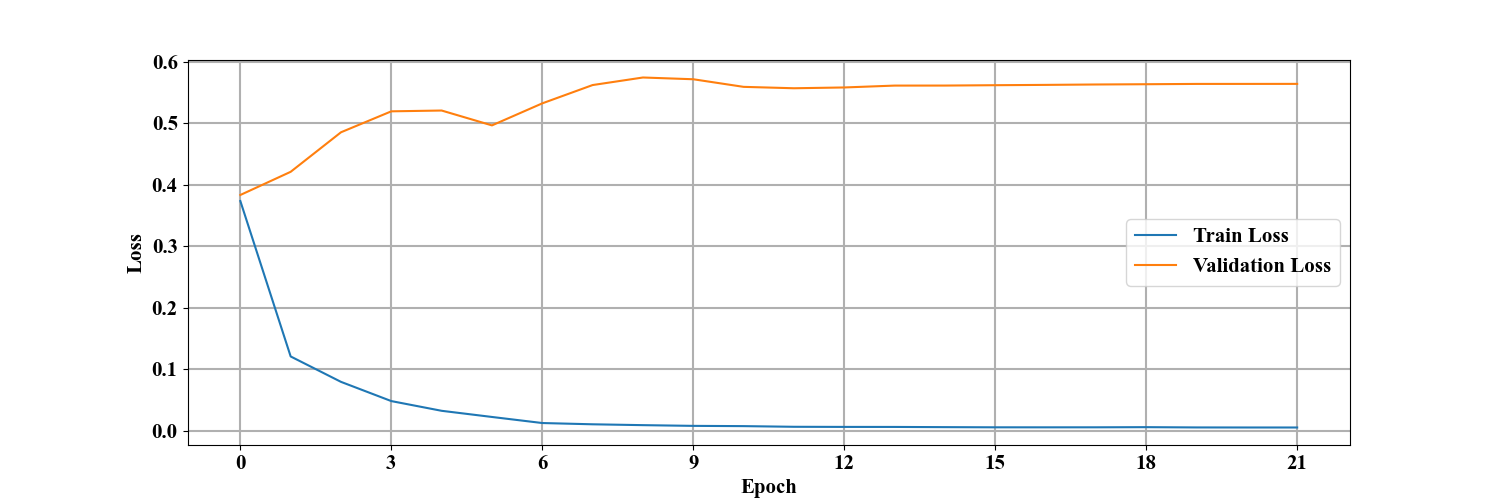
\includegraphics[width=1\linewidth]{images/resultados/nadam_loss.png}}
\caption{Perda do \acrshort{vit} com NAdam.}
\label{fig:nadam_loss}
\end{figure}

Fazendo a mesma análise para a taxa de aprendizagem de 1x10$^{-6}$, onde a acurácia de validação foi um pouco menor, pode-se notar algumas semelhanças e diferenças.
Ainda houve uma diferença significativa entre as acurácias de treino e validação, com a acurácia de treino estabilizando em torno de 0,984, enquanto a acurácia de validação ficou em aproximadamente 0,832.

Entretanto, a curva de perda apresentou melhorias.
Tanto a curva de treino quanto a curva de validação tenderam a diminuir, embora a redução da perda na validação não tenha sido tão significativa.
Este modelo não apresentou sinais claros de \textit{overfitting} como o modelo com maior taxa de aprendizagem, mas ainda demonstra potencial para melhorias.

\begin{figure}[tb]
     \centerline{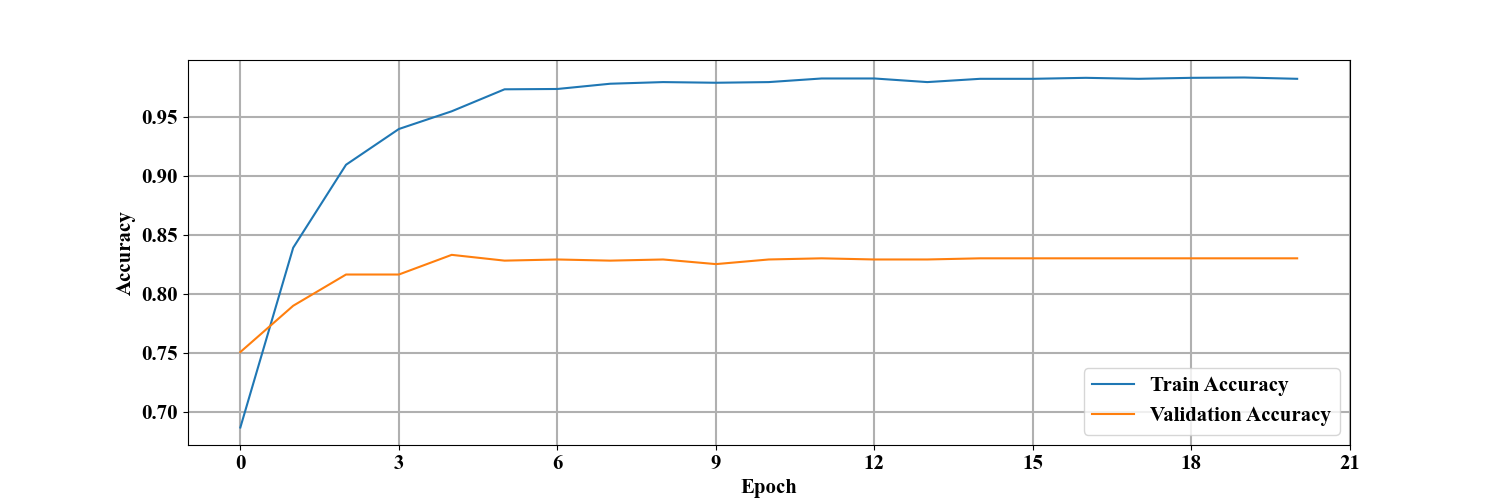
\includegraphics[width=1\linewidth]{images/resultados/nadam_accuracy_1e06.png}}
     \caption{Acurácia do \acrshort{vit} com NAdam e menor taxa de aprendizagem.}
     \label{fig:nadam_acc_1x1006}
\end{figure}
     
\begin{figure}[tb]
     \centerline{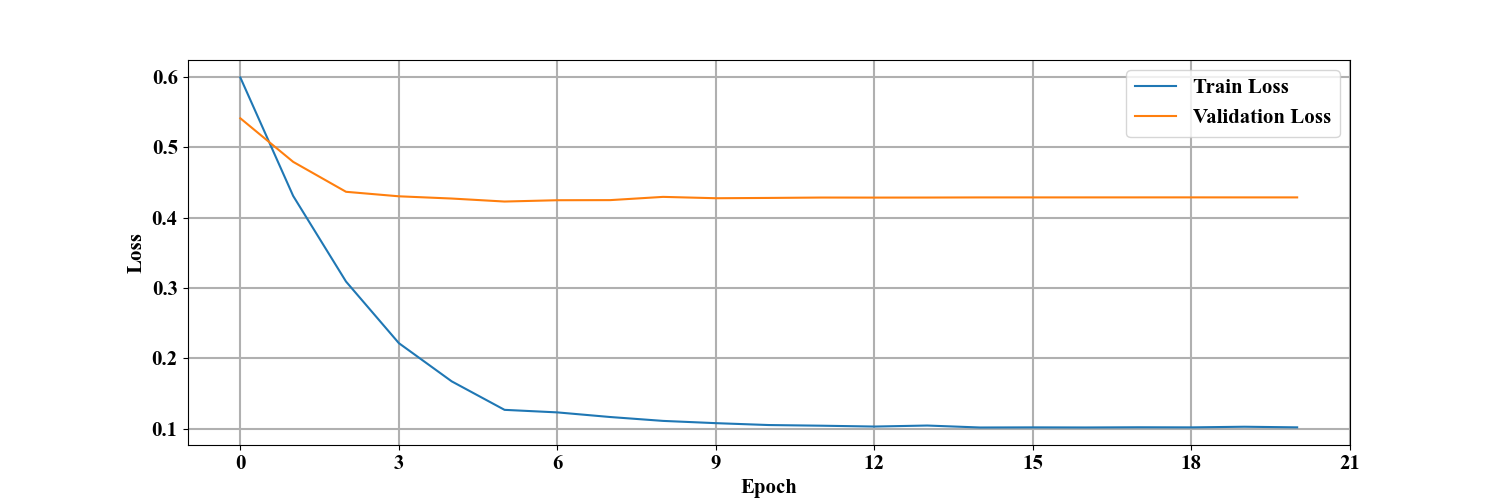
\includegraphics[width=1\linewidth]{images/resultados/nadam_loss_1e06.png}}
     \caption{Perda do \acrshort{vit} com NAdam e menor taxa de aprendizagem.}
     \label{fig:nadam_loss_1x1006}
\end{figure}

Visto que o modelo \acrshort{vit} usando \acrshort{nadam} e taxa de aprendizagem de 1x10$^{-6}$ obteve acurácia de validação semelhante a do modelo com o \acrshort{sgd} de taxa de aprendizagem de 1x10$^{-4}$,
entretanto, teve maior diferença entre as acurácias de treino e validação, assim como redução na função de perda, o modelo com \acrshort{sgd} vai continuar a ser analisado como o melhor modelo, por possuir maior estabilidade.

% ----------------------------------------------------------
\section{Comparações entre cena diurna e noturna}

Para melhor compreender o efeito da iluminação da cena nos resultados de classificação do modelo \cite{piedad2022},
o melhor desempenho do \acrshort{vit} com o otimizador \acrshort{sgd}, descrito na Seção \ref{sec:optimizer}, foi avaliado separadamente em relação às suas métricas para imagens capturadas durante o dia e durante a noite no local.
Os resultados dessa avaliação estão apresentados na Tabela \ref{tab:daynight_acc}.

\begin{table}[tb]
%\resizebox{\columnwidth}{!}
\end{center}
\end{table}

Em contraste com os resultados apresentados e discutidos no Capítulo \ref{cap:trabalhos}, nos quais o modelo exibiu desempenho substancialmente superior em imagens diurnas quando comparado às imagens noturnas \cite{piedad2022},
o modelo treinado com o conjunto de dados \acrshort{rfd} demonstrou diferenças menores na acurácia entre imagens capturadas em condições diurnas e noturnas.
Essa maior estabilidade na acurácia pode ser atribuída à redução da claridade das imagens, obtida por meio do pré-processamento aplicado.

% ----------------------------------------------------------
\section{Outros conjuntos de dados}\label{sec:resultados_outros}

O modelo \acrshort{vit} treinado no conjunto \acrshort{rfd} também foi avaliado em dois outros conjuntos de dados,
o \acrfull{efd} \cite{BarzSchroeterMuench2018_1000117723} e o conjunto de dados de Sazara \textit{et al.} \cite{sazara2019}.
O \acrshort{efd} é composto por 327 imagens da classe normalidade e 252 imagens da classe alagamento, totalizando 579 imagens.
Já o conjunto de dados de Sazara \textit{et al.} contém 491 imagens, das quais 238 correspondem à classe normalidade e 253 à classe alagamento.

Observa-se, na Tabela \ref{tab:vitperformance}, que o desempenho do modelo diminuiu ao ser testado nestes conjuntos distintos.
Apesar do aumento na precisão, houve uma queda significativa na acurácia, indicando que o modelo não conseguiu generalizar adequadamente para imagens com diferentes ângulos, qualidade e condições de iluminação.

\begin{table}[tb]
\caption{\label{tab:vitperformance} Performance do \acrshort{vit} em outros conjuntos de dados}
\begin{center}
\begin{tabular}{c|cccc}
\toprule
 Conjunto de Dados & Acurácia & Precisão & Revocação \\
\midrule
     \acrshort{rfd} & 0,826 & 0,863 & 0,778 \\
     EFD & 0,731 & 0,892 & 0,714 \\
     Sazara & 0,744 & 0,903 & 0,674 \\
\bottomrule
\end{tabular}
\end{center}
\end{table}

\pagestyle{ruledheader}
\chapter{Conclusão}\label{cap:conclusoes}

Com o objetivo de criar um modelo de classificação para classificar o estado de alagamento das ruas da cidade do Rio de Janeiro,
esta pesquisa criou um conjunto de dados original de 4620 através de meses de captação e classificação de imagens da cidade do Rio, que está disponibilizado \href{https://github.com/afego/computervision}{neste repositório de GitHub}.
Com este conjunto de dados, foi realizada uma comparação entre as arquiteturas \acrshort{vgg}, \textit{Inception}, \textit{DenseNet}, \textit{MobileNet} e \Acrshort{vit} no problema de detecção de alagamentos
para achar o melhor modelo entre arquiteturas selecionadas para alcançar o objetivo do trabalho.

Os resultados mostraram que o \acrshort{vit} geralmente superou as outras arquiteturas com diferentes taxas de aprendizagem. 
A alteração da intensidade luminosa da imagem teve impacto claro no desempenho do modelo e ajudou a diminuir a diferença da acurácia entre as imagens noturnas e diurnas, 
em comparação aos resultados descritos em Piedad \textit{et al.} \cite{piedad2022}.

O modelo que se destacou, usando \acrshort{sgd} como otimizador e com taxa de aprendizagem de 1e$^{-4}$ foi o melhor não só pelas suas métricas 
mas pela sua maior estabilidade na curva de perda e pela menor discrepância entre acurácia de treino e validação.

Todos os modelos foram treinados utilizando imagens capturadas pelo sistema de câmeras COR, onde o \acrshort{vit} obteve acurácia de 83\%. 
Este trabalho também analisou o modelo obtido em outras fontes de dados, o modelo conseguiu acurácia de 73\% no conjunto de dados \acrshort{efd} \cite{BarzSchroeterMuench2018_1000117723}, 
e de 74\% no conjunto de dados de Sazara \textit{et al.} \cite{sazara2019}.

Ao abordar o complexo problema de classificar imagens de alagamento de uma cidade grande e diversa como o Rio de Janeiro, 
este trabalho conseguiu alcançar seu objetivo de concluir uma abordagem inicial para a classificação automática da situação de alagamento de ruas, 
através de um conjunto de dados original baseado na própria cidade do Rio.

\section{Trabalhos futuros e considerações}

A integração de diferentes conjuntos de dados ao treinamento do modelo pode impactar positivamente seu desempenho.
Embora diferentes quantidades de tráfego tenham sido utilizadas no treinamento, outros eventos que podem ocorrer na rua ou ao seu redor, como manutenção das vias ou construções, 
não foram incluídos no conjunto de dados de treinamento. 
Portanto, essas situações poderiam ser classificadas incorretamente pelo modelo, e imagens desses eventos deveriam ser incluídas no conjunto de dados de treinamento.

Apesar do otimizador \acrshort{sgd} inicialmente escolhido apresentar melhor desempenho, 
os resultados com o \acrshort{nadam} mostram que mais estudos sobre a escolha de diferentes valores para os parâmetros do otimizador podem aprimorar o modelo atual.

Além disso, alterações na arquitetura como a criação de novas camadas demonstrado em Agung \textit{et al.} \cite{agung2023}, 
pode melhorar o desempenho do modelo uma vez que eles alcançaram uma precisão de 0,95 para o \textit{MobileNetV2}, 
enquanto este trabalho alcançou uma precisão mais baixa de 0,78 com a mesma arquitetura.

O uso de outros instrumentos de medição, como pluviômetros instalados por toda a cidade, pode ser usado para corroborar as classificações resultantes do modelo gerado. 
No entanto, como o escopo da pesquisa foi o desenvolvimento de um modelo de classificação e algumas ruas não possuem sensores de nível de água, 
esse tipo de análise foi deixada de lado para uma abordagem inicial.

% --- -----------------------------------------------------------------
% --- Referencias Bibliograficas. (Obrigatorio)
% --- -----------------------------------------------------------------
\cleardoublepage

 %para personalização da bibliografia olhar os PDFs na pasta "MANUAIS"
\printbibliography[
   % heading=bibintoc,
    title={REFERÊNCIAS} %TITULO DA SEÇÃO
] 

% --- -----------------------------------------------------------------
% --- Apendice.(Opcional)
% --- -----------------------------------------------------------------
\cleardoublepage
\appendix
% para melhor organização deixar os Anexos e Apêndices na pasta anexos.
\chapter{Tabela de quantidade de images de cada classe para cada câmera identificada pelo seu código}
\label{apendA}

% \begin{table}[h]
%     \centering
%     %\caption{Exemplo de Tabela CSV}
%     \csvautotabular{dados/appendixa.csv}
%     \label{tab:apendA}
% \end{table}

% \begin{figure}[htb]
%     \centerline{
\includegraphics[width=1\linewidth]{images/imagespercameratable.png}}
%     %\caption{Quantidade de imagens de normalidade por câmera disponível.}
%     \label{tab:apendA}
% \end{figure}

% \begin{longtable}{|c|c|c|}
%     \hline
%     \textbf{Câmera} & \textbf{Classe 0} & \textbf{Classe 1} \\  
%     \hline
%     \endfirsthead
    
%     \hline
%     \textbf{Câmera} & \textbf{Classe 0} & \textbf{Classe 1} \\  
%     \hline
%     \endhead
    
%     \csvreader[head to column names]{dados/appendixa.csv}{}%
%     {\csvcoli & \csvcolii & \csvcoliii \\}%
% \end{longtable}

\begin{longtable}{|c|c|c|c|c|c|}
    \hline
    \textbf{Câmera} & \textbf{Classe 0} & \textbf{Classe 1} & \textbf{Câmera} & \textbf{Classe 0} & \textbf{Classe 1}\\  
    \hline
    \endfirsthead
    
    \hline
    \textbf{Câmera} & \textbf{Classe 0} & \textbf{Classe 1} & \textbf{Câmera} & \textbf{Classe 0} & \textbf{Classe 1}\\  
    \hline
    \endhead
    
    \csvreader[head to column names]{dados/appendixa_new.csv}{}%
    {\csvcoli & \csvcolii & \csvcoliii & \csvcoliv & \csvcolv & \csvcolvi\\}%
\end{longtable}

% Este apêndice apresenta informações complementares.
% Elemento opcional. 
% O(s) apêndice(s) são identificados por letras maiúsculas consecutivas, travessão e pelos respectivos títulos. 
% Excepcionalmente utilizam-se letras maiúsculas dobradas, na identificação, quando esgotadas as 23 letras do alfabeto (ABNT, 2005).





%\chapter{ANEXO A – TÍTULO DO ANEXO}
\label{lab:anexoA}

"Elemento opcional. O(s) anexo(s) são identificados por letras maiúsculas consecutivas, travessão e pelos respectivos títulos. Excepcionalmente utilizam-se letras maiúsculas dobradas, na identificação dos anexos, quando esgotadas as 23 letras do alfabeto" (ABNT, 2005).


\end{document}

